%  PLEASE DO NOT REMOVE OR CHANGE THIS BLOCK
%  ===========================================================
%
%  A LaTeX Template for Typesetting Theses in Persian
%  By: Mohammad Faraji
%  ===========================================================
%%%% تست شده با تکلایو 2025 
\documentclass[fleqn,a4paper, 12pt, oneside]{report}

\usepackage[paperheight=297mm,paperwidth=210mm,top=25mm, bottom=25mm, left=25mm, right=25mm]{geometry}

\usepackage{lipsum}
\usepackage{draftwatermark}
\SetWatermarkScale{1.1}

%%________________________

\SetWatermarkText{\rotatebox{-45}{
\includegraphics{figures/UOK.png}}}
%___________________________________
\usepackage[subfigure]{tocloft}
%\usepackage[nottoc,notlof,notlot]{tocbibind}
\usepackage{notoccite}
\usepackage{cite}
\usepackage{subfigure}
\usepackage[all]{xy} 
\usepackage{amsmath,amsthm,amssymb,graphicx,tikz,fancyhdr,hyperref} 
\usepackage{mathrsfs,color,xspace,pdflscape} 
\usepackage{bbm}
\usepackage{fancybox}
\usepackage{listings}
\usepackage{multicol} % for multiple columns
\usepackage{zref-perpage}
\usepackage{subfloat}
\zmakeperpage{footnote}
%%%%%%%%%%%%%%%%%%%%%%%
\usepackage{makeidx}
\usepackage{float}
\usepackage[font=scriptsize]{caption}
\usepackage{indentfirst}
\usepackage[nottoc,notlof,notlot]{tocbibind}
\usepackage{setspace}	
\usepackage{sectsty}
\usepackage{fontspec}
\usepackage[labelfont=bf]{caption}
\usepackage{titlesec}
\usepackage{etoolbox}
\graphicspath{{images/}}
\usepackage{unicode-math}
\usepackage{booktabs}
\usepackage{algorithm}
\usepackage{algorithmic}
\usepackage{multirow}
\usepackage{amsfonts}
\usepackage{graphicx}
\usepackage{xcolor}
\usepackage{caption}  % For \caption 
\captionsetup{font=normalsize, skip=1cm}
\usepackage{ptext}
\usepackage{graphicx}
\usepackage{caption}
\usepackage{booktabs}

\newcommand{\mysubfig}[2]{%
	\begin{minipage}[b]{0.3\textwidth}
		\centering
		\includegraphics[width=\textwidth]{#1}
		\caption*{\centering #2}
	\end{minipage}\hfill
}
\usepackage[extrafootnotefeatures]{xepersian}
\usepackage[perpagefootnote=on]{xepersian}
%%%%%%%%%%%%%%%%%%% دستور رنگی کردن لینک‌ها %%%%%%%%%%%%%
%\usepackage{tocloft}

%
\hypersetup{colorlinks=true,linkcolor=black,citecolor=blue,filecolor=magneta,urlcolor=cyan}
\usepackage{fancyhdr}
%       
\newcommand\customfont[1]{{\usefont{T1}{custom}{m}{n} #1 }}
\setlatintextfont[Scale=0.95]{Times New Roman}
\deflatinfont\TNRT[Scale=1.14]{Times New Roman}
\settextdigitfont{IRXLotus}
\settextfont[Scale=1]{XB Titre}
%%%%%%%%%%%%%%%%%%%%%%%%%%%%%%%%%%%%%%%%%%%%%%%%%%%%
\defpersianfont\nastaliq[Scale=1.35]{IranNastaliq}
\defpersianfont\titr[Scale=1.1]{XB Titre}
%%%%%---> B Zar <----%%%%%%%
\defpersianfont\BZarT[Scale=1.34]{XB Zar}
\defpersianfont\BZarTNKS[Scale=1.42]{XB Zar}
\defpersianfont\BZarFTN[Scale=1.17]{XB Zar}
\defpersianfont\BZarTTN[Scale=1.09]{XB Zar}
\defpersianfont\BZarF[Scale=1]{XB Zar}
\defpersianfont\BZarELVN[Scale=0.09]{XB Zar}
%%%%%---> B Zar <----%%%%%%%

%%%%%---> Bold Fonts <----%%%%%%%

\defpersianfont\BZarboldSXTN[Scale=1.33]{XB Zar Bold}
\defpersianfont\BZarboldFTN[Scale=1.16]{XB Zar Bold}
\defpersianfont\BZarboldTTN[Scale=1.08]{XB Zar Bold}
\defpersianfont\BZarboldTLV[Scale=1]{XB Zar Bold}
\defpersianfont\BZarboldE[Scale=0.9]{XB Zar Bold}
\defpersianfont\BNazboldEGT[Scale=1.5]{B Nazanin Bold}
%%%%%---> Bold Fonts Zar <----%%%%%%%

%%%%%---> B Nazanin <----%%%%%%%
\defpersianfont\BNazF[Scale=1.2]{IRNazanin}
\defpersianfont\BNazTTN[Scale=1.09]{IRNazanin}
\defpersianfont\BNazEGT[Scale=1.5]{IRNazanin}
%%%%%---> B Nazanin <----%%%%%%%
%%%%%%%%%%%%%%%%%%%%%%%%%%%%%%%%%%%%%%%%%%%%%%%%%%%%
%لطفا دستورات زیر را تغییر ندهید. 
\newcommand\englishgloss[2]{#2\dotfill\lr{#1}\\}
\newcommand\persiangloss[2]{#1\dotfill\lr{#2}\\}
\renewcommand\proofname{\textbf{برهان}}
\renewcommand{\bibname}{منابع}
%%%%%%%%%%%%%%%%%%%%%%%

\newenvironment{localsize}[1]
{%
	\clearpage
	\let\orignewcommand\newcommand
	\let\newcommand\renewcommand
	\makeatletter
	\input{bk#1.clo}%
	\makeatother
	\let\newcommand\orignewcommand
}
{%
	\clearpage
}



% تعریف و نحوه ظاهر شدن عنوان قضیه‌ها، تعریف‌ها، مثال‌ها و ...
\theoremstyle{definition}
\newtheorem{Alg}{الگوریتم }[section]
\newtheorem{Taz}{تذکر }[section]
\newtheorem{dfn}{تعریف}[section]
\newtheorem{thm}{قضیه}[section]
\newtheorem{lem}{لم}[section]
\newtheorem{pro}{گزاره}[section]
\newtheorem{cor}{نتیجه}[section]
\newtheorem{nok}{نکته}[section]
\newtheorem{rem}{توجه}[section]
\newtheorem{exa}{مثال}[section]
\newtheorem{esb}{اثبات}[section]
\renewcommand{\bibname}{منابع}
\DeclareMathOperator{\ess}{ess}
% شما می‌توانید عناوین را به دلخواه تغییر دهید. به طور مثال، به جای عبارت 
%\newtheorem{thm}{قضیه}
%می‌توان نوشت 
%\newtheorem{theorem}{قضیه}
% البته باید توجه داشت که در کل پایان‌نامه هر جا بخواهید قضیه بنویسید باید از \begin{theorem} و \end{theorem} استفاده شود.
%%%%%%%%%%%%%%%%%%%%%%%%%%%%%%%%%%%%%%%%%%%%%%%%%%%%
%اگر می‌خواهید پایان‌نامه‌ها‌یتان دارای سرفصل باشد و شماره‌گذاری صفحات بالای هر صفحه قرار گیرد، این سه دستور زیر را فعال کنید.
%\pagestyle{fancy}
%\cfoot{}
%\lhead{\thepage}
%%%%%%%%%%%%%%%%ترتیبی کردن عناوین
\makeatletter
\bidi@patchcmd{\@makechapterhead}{\thechapter}{\tartibi{chapter}}
{\typeout{Suceeded}}{\typeout{Failed}}
\makeatother
\chapterfont{\raggedright}
%از این قسمت به بعد، پایان‌نامه شروع می‌شود، بنابراین هر علامت یا هر حرفی نوشته شود در پایان‌نامه چاپ خواهد شد. 
%%% وارد کردن بسته‌های مورد نیاز
% بسته ای برای رنگی کردن لینک ها و فعال سازی لینک ها در یک نوشتار، بسته hyperref باید جزو آخرین بسته‌هایی باشد که فراخوانی می‌شود. 
\usepackage{hyperref}

% بسته‌ای برای وارد کردن واژه نامه در متن، این بسته باید بعد از hyperref حتما صدا زده شود. 
\usepackage[xindy,acronym,nonumberlist=true]{glossaries}

% در مورد تقدم و تاخر وارد کردن بسته ها تنها باید به چند نکته دقت کرد:
% الف) بسته xepersian حتما حتما باید آخرین بسته ای باشد که فراخوانی می شود
% ب) بسته hyperref جزو آخرین بسته هایی باید باشد که فراخوانی می شود.
% ج) بسته glossaries حتما باید بعد از hyperref فراخوانی شود. 
\usepackage{xepersian}
\settextfont{XB Niloofar}
% Custom underline for Persian digits with correct direction
\newcommand{\persianunderline}[1]{%
	\tikz[baseline=(X.base)]{
		\node[inner sep=0pt, anchor=base, font=\normalfont\settextdigitfont{IRXLotus}] (X) {#1};
		\draw[thick] 
		\draw[line width=0.4pt] 
		([yshift=-0.5ex]X.south west) -- ([yshift=-0.5ex]X.south east);
	}%
}

%%%%%% ============================================================================================================

%%% تنظیمات مربوط به بسته  glossaries
%%% تعریف استایل برای واژه نامه فارسی به انگلیسی، در این استایل واژه‌های فارسی در سمت راست و واژه‌های انگلیسی در سمت چپ خواهند آمد. از حالت گروه ‌بندی استفاده می‌کنیم، 
%%% یعنی واژه‌ها در گروه‌هایی به ترتیب حروف الفبا مرتب می‌شوند، مثلا:
%%% الف
%%% افتصاد ................................... Economy
%%% اشکال ........................................ Failure
%%% ش
%%% شبکه ...................................... Network
\newglossarystyle{myFaToEn}{%
	\renewenvironment{theglossary}{}{}
	\renewcommand*{\glsgroupskip}{\vskip 10mm}
	\renewcommand*{\glsgroupheading}[1]{\subsection*{\glsgetgrouptitle{##1}}}
	\renewcommand*{\glossentry}[2]{\noindent\glsentryname{##1}\dotfill \glsentrytext{##1}
		
	}
}

%% % تعریف استایل برای واژه نامه انگلیسی به فارسی، در این استایل واژه‌های فارسی در سمت راست و واژه‌های انگلیسی در سمت چپ خواهند آمد. از حالت گروه ‌بندی استفاده می‌کنیم، 
%% % یعنی واژه‌ها در گروه‌هایی به ترتیب حروف الفبا مرتب می‌شوند، مثلا:
%% % E
%%% Economy ............................... اقتصاد
%% % F
%% % Failure................................... اشکال
%% %N
%% % Network ................................. شبکه

\newglossarystyle{myEntoFa}{%
	%%% این دستور در حقیقت عملیات گروه‌بندی را انجام می‌دهد. بدین صورت که واژه‌ها در بخش‌های جداگانه گروه‌بندی می‌شوند، 
	%%% عنوان بخش همان نام حرفی است که هر واژه در آن گروه با آن شروع شده است. 
	\renewenvironment{theglossary}{}{}
	\renewcommand*{\glsgroupskip}{\vskip 10mm}
	\renewcommand*{\glsgroupheading}[1]{\begin{LTR} \subsection*{\glsgetgrouptitle{##1}} \end{LTR}}
	%%% در این دستور نحوه نمایش واژه‌ها می‌آید. در این جا واژه فارسی در سمت راست و واژه انگلیسی در سمت چپ قرار داده شده است، و بین آن با نقطه پر می‌شود. 
	\renewcommand*{\glossentry}[2]{\noindent\glsentrytext{##1}\dotfill\space \glsentryname{##1}
		
	}
}

%%% تعیین استایل برای فهرست اختصارات
\newglossarystyle{myAbbrlist}{%
	%%% این دستور در حقیقت عملیات گروه‌بندی را انجام می‌دهد. بدین صورت که اختصارات‌ در بخش‌های جداگانه گروه‌بندی می‌شوند، 
	%%% عنوان بخش همان نام حرفی است که هر اختصار در آن گروه با آن شروع شده است. 
	\renewenvironment{theglossary}{}{}
	\renewcommand*{\glsgroupskip}{\vskip 10mm}
	\renewcommand*{\glsgroupheading}[1]{\begin{LTR} \subsection*{\glsgetgrouptitle{##1}} \end{LTR}}
	%%% در این دستور نحوه نمایش اختصارات می‌آید. در این جا حالت کوچک اختصار در سمت چپ و حالت بزرگ در سمت راست قرار داده شده است، و بین آن با نقطه پر می‌شود. 
	\renewcommand*{\glossentry}[2]{\noindent\glsentrytext{##1}\dotfill\space \Glsentrylong{##1}
		
	}
	%%% تغییر نام محیط abbreviation به فهرست اختصارات
	\renewcommand*{\acronymname}{\rl{فهرست اختصارات}}
}

%%% برای اجرا xindy بر روی فایل .tex و تولید واژه‌نامه‌ها و فهرست اختصارات و فهرست نمادها یکسری  فایل تعریف شده است.‌ Latex داده های مربوط به واژه نامه و .. را در این 
%%%  فایل‌ها نگهداری می‌کند. مهم‌ترین option‌ این قسمت این است که 
%%% عنوان واژه‌نامه‌ها و یا فهرست اختصارات و یا فهرست نمادها را می‌توانید در این‌جا مشخص کنید. 
%%% در این جا عباراتی مثل glg، gls، glo و ... پسوند فایل‌هایی است که برای xindy بکار می‌روند. 
\newglossary[glg]{english}{gls}{glo}{واژه‌نامه انگلیسی به فارسی}
\newglossary[blg]{persian}{bls}{blo}{واژه‌نامه فارسی به انگلیسی}
\makeglossaries
\glsdisablehyper
%%% تعاریف مربوط به تولید واژه نامه و فهرست اختصارات و فهرست نمادها
%%%  در این فایل یکسری دستورات عمومی برای وارد کردن واژه‌نامه آمده است.
%%%  به دلیل این‌که قرار است این دستورات پایه‌ای را بازنویسی کنیم در این‌جا تعریف می‌کنیم. 
\let\oldgls\gls
\let\oldglspl\glspl

\makeatletter

\renewrobustcmd*{\gls}{\@ifstar\@msgls\@mgls}
\newcommand*{\@mgls}[1] {\ifthenelse{\equal{\glsentrytype{#1}}{english}}{\oldgls{#1}\glsuseri{f-#1}}{\lr{\oldgls{#1}}}}
\newcommand*{\@msgls}[1]{\ifthenelse{\equal{\glsentrytype{#1}}{english}}{\glstext{#1}\glsuseri{f-#1}}{\lr{\glsentryname{#1}}}}

\renewrobustcmd*{\glspl}{\@ifstar\@msglspl\@mglspl}
\newcommand*{\@mglspl}[1] {\ifthenelse{\equal{\glsentrytype{#1}}{english}}{\oldglspl{#1}\glsuseri{f-#1}}{\oldglspl{#1}}}
\newcommand*{\@msglspl}[1]{\ifthenelse{\equal{\glsentrytype{#1}}{english}}{\glsplural{#1}\glsuseri{f-#1}}{\glsentryplural{#1}}}

\makeatother

\newcommand{\newword}[4]{
	\newglossaryentry{#1}     {type={english},name={\lr{#2}},plural={#4},text={#3},description={}}
	\newglossaryentry{f-#1} {type={persian},name={#3},text={\lr{#2}},description={}}
}

%%% بر طبق این دستور، در اولین باری که واژه مورد نظر از واژه‌نامه وارد شود، پاورقی زده می‌شود. 
\defglsentryfmt[english]{\glsgenentryfmt\ifglsused{\glslabel}{}{\LTRfootnote{\glsentryname{\glslabel}}}}

%%% بر طبق این دستور، در اولین باری که واژه مورد نظر از فهرست اختصارات وارد شود، پاورقی زده می‌شود. 
\defglsentryfmt[acronym]{\glsentryname{\glslabel}\ifglsused{\glslabel}{}{\LTRfootnote{\glsentrydesc{\glslabel}}}}
\LTRfootmarkstyle{#1\textsubscript{.}}
%%%%%% ============================================================================================================

%%============================ دستور برای قرار دادن فهرست اختصارات 
\newcommand{\printabbreviation}{
	\cleardoublepage
	\phantomsection
	\baselineskip=.75cm
	%% با این دستور عنوان فهرست اختصارات به فهرست مطالب اضافه می‌شود. 
	\addcontentsline{toc}{chapter}{فهرست اختصارات}
	\setglossarystyle{myAbbrlist}
	\begin{LTR}
		\Oldprintglossary[type=acronym]	
	\end{LTR}
	\clearpage
}%

\newcommand{\printacronyms}{\printabbreviation}
%%% در این جا محیط هر دو واژه نامه را باز تعریف کرده ایم، تا اولا مشکل قرار دادن صفحه اضافی را حل کنیم، ثانیا عنوان واژه نامه ها را با دستور addcontentlist وارد فهرست مطالب کرده ایم.
\let\Oldprintglossary\printglossary
\renewcommand{\printglossary}{
	\let\appendix\relax
	%% تنظیم کننده فاصله بین خطوط در این قسمت
	\clearpage
	\phantomsection
	%% این دستور موجب این می‌شود که واژه‌نامه‌ها در  حالت دو ستونی نوشته شود. 
	%	\twocolumn{}
	%% با این دستور عنوان واژه‌نامه به فهرست مطالب اضافه می‌شود. 
	\addcontentsline{toc}{chapter}{واژه نامه انگلیسی به فارسی}
	\setglossarystyle{myEntoFa}
	\Oldprintglossary[type=english]
	
	\clearpage
	\phantomsection
	%% با این دستور عنوان واژه‌نامه به فهرست مطالب اضافه می‌شود. 
	\addcontentsline{toc}{chapter}{واژه نامه فارسی به انگلیسی}
	\setglossarystyle{myFaToEn}
	\Oldprintglossary[type=persian]
	\onecolumn{}
}%

\makeatletter
\def\LTRfootnotetext{\@ifnextchar[\@xLTRfootnote{\stepcounter\@mpfn
		\protected@xdef\@thefnmark{\persianfont}%
		\@LTRfootnotetext}}
\patchcmd{\@LTRfootnotetext}{\tiny}{\tiny\sffamily}{}{}
\makeatother

\makeatletter
\newcommand*{\Computebaselinestretch}[1]{%
	\strip@pt\dimexpr\number\numexpr\number\dimexpr#1\relax*65536/\number\dimexpr\baselineskip\relax\relax sp\relax
}
\makeatother
\linespread{\Computebaselinestretch{1cm}}
%%%%%% ============================================================================================================

\input{MyGlossy.tex}
\begin{document}
	
	\BNazF
\section*{\textcolor{red}{\textbf{تصویر فارسی جلد در این صفحه قرار میگیرد.}}}
\thispagestyle{empty}
\DraftwatermarkOptions{stamp=false}
	
	%\linespread{\Computebaselinestretch{1cm}}
\thispagestyle{empty}
\begin{figure}[ht]
	\vspace{7cm}
	\centerline{
\includegraphics[height=4.5cm]{figures/besm.png}}
\end{figure} 


%هر عکس یا تصویری که می‌خواهید در متن باشد، باید در پوشه‌ای که این قالب قرار دارد، گذاشته شود، در غیر اینصورت عکس نامبرده را نمی‌شناسد.
%%%%%%%%%%%%  صفحه عنوان فارسی و روی جلد
\newpage
\DraftwatermarkOptions{stamp}

\thispagestyle{empty}
\begin{center}
		\vspace*{-1.5cm}
	\begin{figure}[ht]
		\centerline{
\includegraphics[height=2.5cm]{figures/UOK_LOGO.png}}
	\end{figure}
	\vspace*{-0.6cm}
	\BZarboldFTN{\large دانشگاه‌ کردستان}\
	\vspace*{-0.2cm}\\
	\BZarboldTTN{ دانشکده مهندسی}
	\vspace*{-0.2cm}\\
	\BZarboldTLV{ گروه مهندسی نرم‌افزار کامپیوتر}
	\vspace*{1cm}
	
	
	\BZarboldTLV{\fontsize{14}{0}
		پایان‌نامه
		 کارشناسی ارشد
		رشته کامپیوتر گرایش  هوش‌مصنوعی و رباتیکز
	}\\
	\vspace*{0.5cm}
	\BZarboldFTN{\Large عنوان:}\\
	\BZarboldSXTN{
	انتخاب ویژگی چندبرچسبه با استخراج همبستگی برچسب‌ سراسری و محلی
	}\\
	\vspace*{1cm}
	\BZarboldTLV{پژوهشگر:}\\
	\BZarboldFTN{
	محمد فرجی
	}\\
	\vspace*{1cm}
	\BZarboldTLV{استاد راهنما:}\\
	\BZarboldFTN{\textbf{
دکتر فردین اخلاقیان‌طاب
	}}\\
	
	\vspace*{1cm}
	\BZarboldTLV{استاد مشاور :}\\
	\BZarboldFTN{
سیدامجد سیدی
	}\\	
	\vspace*{2cm}
	\BZarF{
		شهریور 1402
	}
\end{center}
%%%%%%%%%%
	%% evaluation page...
	\thispagestyle{empty}

\begin{center}
	
	
	
	\BZarboldFTN{كليه‌ی‌ حقوق‌ مادي‌ و معنوی مترتب‌ بر نتايـج‌ مطالعات، \\
		ابتكارات‌ و نوآوري‌هاي‌ ناشي‌ از تحقيق‌ موضوع ‌\\
		اين‌ پايان‌‌نامه‌ متعلق‌ به‌ دانشـگاه‌ کردستان است‌.
	}
\end{center}
\newpage
\BNazF
\thispagestyle{empty}
{
	\baselineskip=0.8cm
	
	\begin{center}
		***تعهد نامه***
		\vspace*{-0.5cm}\\
		
	\end{center}	
	
		اینجانب محمد فرجی دانشجوی کارشناسی ارشد رشته مهندسی کامپیوتر، گرایش هوش مصنوعی و رباتیکز دانشگاه کردستان، دانشکده مهندسی گروه مهندسی نرم‌افزار کامپیوتر تعهد می‌نمایم که محتوای این پایان‌نامه نتیجه تلاش و تحقیقات خود بوده و از جایی کپی‌برداری نشده و به پایان رسانیدن آن نتیجه تلاش و مطالعات مستمر اینجانب و راهنمایی و مشاوره اساتید بوده است. 
	%		\vspace*{0.3cm}\\
	%		\hspace*{0.3cm}
	\begin{flushleft}
		با تقدیم احترام‎\\محمد فرجی \\ 24 فروردین 1404 
	\end{flushleft}
	\vspace*{-0.3cm}
	
	
	\newpage
	\thispagestyle{empty}
	\begin{center}
		
		
		\BNazF{\textbf{باسمه تعالی}}\\
		$ \star $ \hspace*{-0.1cm}
		\BNazF{
			\textbf{
				تعهدنامه دانشجویان تحصیلات تکمیلی دانشگاه کردستان
				در انجام پایان‌نامه 
		}}
		$ \star $ \hspace*{-0.1cm} \\
		\vspace*{-0.2cm}
		%		\hspace*{2.5cm}
		%		\Tera{
			%			(لازم است به عنوان صفحه اول پروپوزال و به عنوان چهارمین برگ پایان‌نامه و پس از صفحه مشخصات پایان‌نامه بوده و به دقت مطالعه و امضا شود) 
			%		}
	\end{center}
	
	اینجانب محمد فرجی دانشجوی مقطع کارشناسی ارشد رشته مهندسی کامپیوتر گرایش هوش مصنوعی و رباتیکز متعهد می‌شوم:
	
	\begin{enumerate}
		\item صداقت، امانتداری و بی طرفی را در انجام پژوهش  و انتشار نتایج حاصل از آن رعایت نمایم.
		\item در نگارش نتیجه پژوهشهای حاصل از موضوع پایان‌نامه از بازنویسی نوشته‌های دیگران بدون ذکر منبع، بازی با الفاظ، زیاده‌‌نویسی، كلی‌گویی و جزماندیشی و تصرف گرایی پرهیز نمایم و نتایج پژوهشی خود را در موعد مقرر و با اطلاع استاد راهنما منتشر نمایم.
		
		\item  تمامی یافته‌های مستخرج از پایان‌نامه متعلق به دانشگاه کردستان بوده و لازم است در کلیه مقالات مستخرج از آنها نام دانشگاه کردستان را تحت عنوان (دانشجوی دانشگاه کردستان) یا 				(دانش‌آموخته دانشگاه کردستان) ذکر نمایم.
		
		\item در انتشار مقالات نام استاد (استادان) راهنما و استاد (استادان) مشاور را در لیست مولفین مقاله ذکر نمایم و از آوردن اسامی افرادی که نقش موثری در انجام پژوهش نداشته‌اند، جداً خودداری نمایم.
		
		\item در بخش سپاسگزاری مقاله، از تمامی افراد و سازمان‌هایی که در اجرای پژوهش مساعدتی مبذول داشته‌اند با ذکر نوع مشارکت تشکر و قدردانی نمایم.
		\item از انتشار همپوشان یا ارسال همزمان یک مقاله به چند مجله و یا ارسال مجدد مقاله چاپ شده به مجلات دیگر خودداری نمایم.
		\item  در صورت عدم رعایت موارد مذکور، دانشگاه کردستان مجاز خواهد بود تا برابر مقررات اقدام نماید.
		
		
	\end{enumerate}
	\begin{center}
		\textbf{\BNazF{امضاء دانشجو}}
	\end{center}
	
	\begin{table}[!ht] 
		\begin{center}
			\scalebox{0.70}{
				\begin{tabular}{||r||}
					\hline 
					\hline
					\\
					$ 
					\text{
						\BNazF{
							\textbf{
								دستور العمل نحوه برخورد با موارد تخطی دانشجویان تحصیلات تکمیلی در هنگام انتشار نتایج پژوهش 
							}
						}
					}
					$ 
					\\
					$ 
					\text{
						1-  درموارد زیر دانشگاه کردستان با مجله مربوطه مکاتبه و درخواست خارج نمودن مقاله را نموده و موضوع را به محل کار یا تحصیل بعدی 
					}
					$ \\
					$ 
					\text{
						دانشجو اطلاع خواهد داد. 
					}
					$ \\
					$ 
					\text{
						الف: چاپ مقاله بدون اطلاع و تأیید استادان راهنما
					}
					$ \\
					$ 
					\text{
						ب: چاپ نتایج حاصل از پژوهش های انجام شده در دانشگاه کردستان بدون ذکر نام دانشگاه 
					}
					$ \\
					$ 
					\text{
						2- در صورت احراز تخلف از سایر موارد درج شده در تعهد نامه دانشجویی، دانشگاه ضمن مکاتبه با مجله مربوطه، حسب مورد تصمیم‌گیری
					}
					$ \\
					$ 
					\text{
						خواهد نمود.
					}
					$ \\
					$ 
					\text{
					}
					$ \\
					\hline
					\hline
			\end{tabular}}
			
		\end{center}
	\end{table}
}
	%
	
	%% submission page...
	
\thispagestyle{empty}
\begin{center}
	\vspace*{-1.5cm}
	\begin{figure}[ht]
		\centerline{
\includegraphics[height=2.5cm]{figures/UOK_LOGO.png}}
	\end{figure}
	\vspace*{-0.5cm}
	\BZarboldFTN{\large دانشگاه‌ کردستان}\\
	\vspace*{-0.3cm}
	\BZarboldTTN{ دانشکده مهندسی}\\
	\vspace*{-0.3cm}
	\BZarboldTLV{ گروه مهندسی نرم‌افزار کامپیوتر}\\
	\vspace*{2cm}
	
	
	{\fontsize{14}{0}
		پایان‌نامه
		کارشناسی ارشد
		رشته مهندسی کامپیوتر گرایش  هوش مصنوعی و رباتیکز
	}\\
	\vspace*{1cm}
	\BZarboldFTN{\Large عنوان:}\\
	\BZarboldSXTN{
	انتخاب ویژگی چندبرجسبه با استخراج همبستگی برچسب‌ سراسری و محلی
	}\\
	\vspace*{1cm}
	\BZarboldTLV{پژوهشگر:}\\
	\BZarboldFTN{
محمد فرجی
	}\\
\end{center}
\BZarF{
	در تاریخ 
	21٫06٫1402
	توسط کمیته تخصصی و هیات داوران زیر مورد بررسی قرار گرفت و با
	%%%%%%%%%%%%%%%%%%%%%
	% نمره 
	%$ ......... $
	%و 
	%برای دانشجویان دکتری باید نمره حتما وارد شود.
	%%%%%%%%%%%%%%%%%%%%%
	درجه 
	\textbf{عالی}
	به تصویب رسید.
}
%\vspace*{-0.5cm}\\
%%%%
\begin{table}[!ht]
	\renewcommand{\arraystretch}{2}
	\raggedleft{
		%\scalebox{0.7}{
			\begin{tabular}{rrcc}
				$ \underline{\text{هیات داوران}} $ & $ \underline{\text{نام و نام‌خانوادگی }} $ & $ \hspace*{0.2cm} \underline{\text{مرتبه علمی }} \hspace*{0.2cm} $ & $ \underline{\text{امضاء }} \hspace*{0.5cm} $ \\
				$ \text{1. استاد راهنما } $  &  $ \text{دکتر فردین اخلاقیان طاب }                           $  &  $ \text{\textcolor{black}{دانشیار}}  $  &  \\
				$ \text{2. استاد مشاور} $ & $ \text{سید امجد سیدی}                                    $  &  $ \text{\textcolor{black}{استادیار}} $  &  \\
				$ \text{3. استاد داور \textcolor{black}{خارجی}} $  	 & $ \text{دکتر محسن رمضانی}           $  &  $ \text{\textcolor{black}{استادیار}} $  &  \\
				$ \text{4. استاد داور \textcolor{black}{داخلی}} $   	& $ \text{دکتر روجیار پیرمحمدیانی} $  &  $ \text{\textcolor{black}{استادیار}} $  &  \\
				% $ \text{مهر و امضاء مدیر گروه } $ &    & $ \text{معاون آموزشی و تحصیلات تکمیلی دانشکده} $  & 
		\end{tabular}}
		%}
\end{table}

\hspace*{-0.8cm}
مهر و امضاء مدیر گروه
\hspace*{2.9cm}
مهر و امضاء معاون آموزشی و تحصیلات تکمیلی دانشکده

\hspace*{-0.8cm}

\hspace*{3.15cm}


%%%
%%%%%%%%%%
%%%%%%%%%%%%%%%%%%%%%%%%%%%%%%%%%%%%%%%
%%%%%%%%%%%
%توجه: عناوین فارسی و انگلیسی و صفحات واگذاری حقوق و ... در این قالب نوشته نشده و شما باید شیوه‌نامه تدوین پایان‌نامه را برای تنظیم این صفحات از سایت دانشگاه گرفته و با دقت پر نمایید.

	%% acknowledgements page...
	\thispagestyle{empty}
\vspace*{1cm}
{\nastaliq \Large
	{\huge 
		\hspace*{-0.9cm}تقدیم به وجود نازنین  \\
		
		\hspace*{2cm} مادر مهربان و بی‌همتایم‎\\
		\vspace*{0.5cm}
	}
	\huge
	‎\hspace*{5cm} پدر دلسوز و فداکارم ...‎
}


%%%%%%%%%%%%%% صفحه تقدیم و تشکر
\newpage
\thispagestyle{empty}
\vspace*{1cm}
{\nastaliq 
	\begin{center}
		{ \huge{تقدیر و تشکر}}
	\end{center}
}
{\nastaliq\large
	
	سپاس و ستایش مرخدایی را جل و جلاله که آثار قدرت او بر چهره روز روشن، تابان است و انوار حکمت او در دل شب تار، درفشان. آفریدگاری که خویشتن را به شناساند و درهای علم را بر ما گشود و عمری و فرصتی عطا فرمود تا بدان، بنده‌ی ضعیف خویش را در طریق علم و معرفت بیازماید.‎\\‎
	تشکر و سپاس از استاد دانشمند و پرمایه‌ام جناب آقای دکتر فردین اخلاقیان طاب که از محضر پرفیض تدریسشان و علم اندوزیشان بهره‌ها  برده‌ام.‎\\‎
	با امتنان و تشکر بیکران از مساعدت، لطف و دلسوزی‌های بی‌شائبه استاد، دوست و برادر ارجمندم جناب آقای دکتر سیدامجد سیدی که به واقع ریزه‌خوان دانش ایشان بوده و خواهم بود.
	
}

	%
	%% alphabetic page numbering for non-report pages...
	
	\newpage
	%% the abstract page...
	\thispagestyle{empty}
\BZarboldE\section*{چکیده}
\BNazTTN
در حوزه‌های مختلف کاربردی، داده‌های چندبرچسبه با ابعاد بالا بسیار موردتوجه قرار گرفته‌اند که دو چالش مهم شامل: نمونه‌ها با ویژگی‌های بُعد بالا و همچنین تعداد زیادی برچسب را به همراه دارد. در انتخاب ویژگی چندبرچسبه، هدف انتخاب زیرمجموعه‌ای از ویژگی‌ها از یک مجموعه است که برای پیش‌بینی چندین برچسب یا دسته مرتبط با هر نمونه بسیار مناسب می‌باشد. با این‌حال، اغلب روش‌های موجود طبقه‌بندی چندبرچسبه، مواردی چون وابستگی‌های برچسب و توزیع نامتعادل برچسب را نادیده گرفته‌اند، هرچند که دارای بینش‌های ارزشمند برای طراحی الگوریتم‌های مؤثر انتخاب ویژگی چندبرچسبه باشند.
در این پایان‌نامه، یک مدل انتخاب ویژگی پیشنهاد می‌شود که با بهره‌گیری از همبستگی‌های سراسری و محلی برچسب‌ها، ویژگی‌های متمایزکننده در سراسر برچسب‌ها را انتخاب ‌کند. علاوه‌بر‌این، با بازنمایی ماتریس ویژگی و ماتریس برچسب در یک فضای مشترک نهان، همبستگی‌های موجود بین ویژگی‌ها و برچسب‌ها را بدست می‌آورد. در این فضای مشترک، الگوها یا ارتباطات مشترکی که در سراسر چندین ‌برچسب و ویژگی وجود دارد، مشخص می‌شود. تابع پیشنهادی شامل نُرم $\ell_{2,1} $ و یک الگوریتم مبتنی بر تکرار و بهینه‌سازی متناوب ‌است تا ضرایب خلوت مورد نیاز برای انتخاب ویژگی چندبرچسبه را بدست آورد. 
ارزیابی روش پیشنهادی بر روی شش معیار ارزیابی و دوازده مجموعه‌داده انجام شده است و نتایج نشان‌دهنده این است که مدل ارائه شده مؤثر، و عملکرد آن از روش‌های مقایسه‌شده بهتر است. \\
\textbf{کلمات کلیدی :}
انتخاب ویژگی، یادگیری چندبرچسبه، همبستگی برچسب، تجزیه ماتریس نامنفی
	
	% table of content...
	\pagenumbering{alph}
	\addtocontents{toc}{\textbf{عنوان}~\hfill\textbf{صفحه}\vspace*{0.3cm}\par\hrule height 1pt\vskip 1.4pt\hrule height 1pt\par}
	\addtocontents{lof}{\textbf{عنوان}~\hfill\textbf{صفحه}\vspace*{0.3cm}\par\hrule height 1pt\vskip 1.4pt\hrule height 1pt\par}
	\addtocontents{lot}{\textbf{عنوان}~\hfill\textbf{صفحه}\vspace*{0.3cm}\par\hrule height 1pt\vskip 1.4pt\hrule height 1pt\par}
	\renewcommand{\cfttoctitlefont}{\hspace*{\fill}\large\bfseries\underline}
	\renewcommand{\cftaftertoctitle}{\hspace*{\fill}\vspace*{-1.8cm}}
	\renewcommand{\cftlottitlefont}{\hspace*{\fill}\large\bfseries\underline}
	\renewcommand{\cftafterlottitle}{\hspace*{\fill}\vspace*{-1.8cm}}
	\renewcommand{\cftloftitlefont}{\hspace*{\fill}\large\bfseries\underline}
	\renewcommand{\cftafterloftitle}{\hspace*{\fill}\vspace*{-1.8cm}}
	\vspace*{-2.5cm}
	\tableofcontents
	% group the list of figures, list of tables and table of contents in one page...
	\begingroup
	\let\clearpage\relax
	\newpage
	% list of figures...
	\vspace*{-2.5cm}
	\listoffigures
	\newpage
	% list of tables...
	\vspace*{-2.5cm}
	\listoftables
	\endgroup
% درصورت نیاز به پیش تعریف، دستور زیر را فعال نمایید.
	%\include{Chapters/1-pre-intr}
	%%%%%%%%%%%%%%%%%%%%%%%%%%%%%%
	\pagenumbering{arabic}
\twocolumnfootnotes
\titleformat{\chapter}[display]
{\normalfont\Large\BNazboldEGT\centering}
{\vspace*{8cm}{‎\textbf{فصل اول}}}{5pt}{\Large}
\chapter{ \textbf{مقدمه}  }\label{sec1}
\thispagestyle{empty}
\newpage

%%%%%%%%%%%%%%%%%
\section{بیان و اهمیت مسئله}
به دلیل تأثیرات منفی ویژگی‌های با ابعاد بالا\LTRfootnote{High dimentionality features}مانند افزایش پیچیدگی  یادگیری\LTRfootnote{Learning complexity}
\cite{liu2018onlinee,li2017granular}، افزایش تخصیص فضا\LTRfootnote{Heightened space allocation}
\cite{lin2017streaming}
و کاهش کارایی طبقه‌بندها \LTRfootnote{Classification}، توجه به روش‌های انتخاب‌ویژگی\LTRfootnote{Feature selection}روز‌به‌روز بیشتر شده است \cite{gao2018class}. در طول سال‌های اخیر، انتخاب ویژگی به یکی از مسائل مهم تبدیل شده است که تنها با انتخاب ویژگی‌های مرتبط\LTRfootnote{Relevant}و حذف ویژگی‌های تکراری\LTRfootnote{Redundant}و نامربوط\LTRfootnote{Irrelevant}
\cite{huang2017joint,zhu2018multi}،
می‌توان تعداد ویژگی‌ها را کاهش و کارایی مدل را بهبود داد. انتخاب ویژگی در مسائل مختلفی مانند: سیستم‌های توصیه‌گر\LTRfootnote{Recommender systems}، حاشیه‌نویسی تصویر
و ویدئو \LTRfootnote{Video annotation}\cite{hong2013image}، پردازش داده‌های ریزآرایه\LTRfootnote{Microarray data processing}و ژنومیکس\LTRfootnote{Genomics}\cite{xie2021unsupervised} به تدریج درحال گسترش است. از آنجایی که اشیاء در دنیای واقعی در عین حال چندین برچسب\LTRfootnote{Multi-Label}دارند، تحقیقات قابل توجهی در مورد انتخاب ویژگی در این حوزه‌ها انجام شده است. برای مثال در ژنومیکس، یک ژن می‌تواند چندین وظیفه‌ مانند: فتوسنتز\LTRfootnote{Photosynthesis}، تجزیه پروتئین\LTRfootnote{Protein breakdown}و انتقال سیگنال\LTRfootnote{Signal transmission}  \cite{wang2008building} داشته باشد.‎\\
در تحلیل موسیقی\LTRfootnote{Music analysis}، یک قطعه موسیقی می‌تواند همزمان دارای چند احساس مختلف مانند غم، شادی و ترس باشد \cite{trohidis2008multi}. همچنین در دسته‌بندی اخبار یک خبر می‌تواند جزو دسته‌های مختلفی باشد. در یادگیری چندبرچسبه، برخلاف مسائل چندکلاسه\LTRfootnote{Multi-Class}، همبستگی بین برچسب‌ها درنظر گرفته می‌شود. به همین دلیل، علاوه بر فضای ابعاد، استخراج و استفاده از همبستگی برچسب‌ها این مسئله را به یک مسئله \lr{NP-hard} تبدیل کرده است. 

درحال حاضر روش‌های انتخاب ویژگی چندبرچسبه بر روی استخراج همبستگی\LTRfootnote{Extraction of correlation} برچسب-برچسب، وابستگی برچسب-ویژگی و همبستگی ویژگی-ویژگی کار می‌کنند. روش‌های انتخاب ویژگی چندبرچسبه به دو دسته انتقال مسئله\LTRfootnote{Problem transformation}و تطبیق الگوریتم\LTRfootnote{Algorithm adaption}تقسیم می‌شوند\cite{6471714}. در رویکرد اول، مسئله به داده تک‌برچسبه\LTRfootnote{Single-Lable}تبدیل می‌شود و با استفاده از الگوریتم‌های تک‌برچسبه، حل می‌شوند. در رویکرد دوم، محققان تعدادی مدل انطباق الگوریتم ارائه داده‌اند که به‌صورت مستقیم مسائل چندبرچسبه را حل می‌کنند \cite{zhang2022non,jian2016multi}. همبستگی‌های برچسب عمدتاً توسط روش‌های انطباق الگوریتم برای روند انتخاب ویژگی استخراج می‌شوند. 
روش‌های تطبیق الگوریتم نسبت به روش‌های انتقال مسئله، بهینه‌تر هستند زیرا در تبدیل مسئله همبستگی بین برچسب‌ها در‌نظر گرفته‌ نمی‌شود. روش تطبیق الگوریتم به سه رویکرد مرتبه‌اول\LTRfootnote{First-order}، مرتبه‌دوم\LTRfootnote{Second-order}و مرتبه‌بالا\LTRfootnote{High-order}تقسیم می‌شود. در رویکرد مرتبه‌اول همبستگی بین برچسب‌ها درنظر گرفته نمی‌شود و برچسب‌ها مستقل از یکدیگر متصور می‌شوند. در رویکرد مرتبه‌دوم همبستگی جفت برچسب درنظر گرفته می‌شود. در عمل، یک رتبه‌بندی بین برچسب‌های مرتبط و غیرمرتبط خواهیم داشت. در رویکرد مرتبه‌بالا، همبستگی بین یک زیرمجموعه یا کل مجموعه برچسب‌ها درنظر گرفته می‌شود. در یادگیری چندبرچسبه، همبستگی بین برچسب‌ها می‌توانند داده‌های مهمی را ارائه دهند، برای مثال: اگر برچسب‌های اسکیت‌بُرد و برف وجود داشته باشند، به احتمال زیاد برچسب ورزش‌های زمستانی نیز وجود خواهد داشت. به‌طور مشابه اگر برچسب‌های دریا و هوای‌آفتابی وجود داشته باشند، به احتمال زیاد برچسب برف وجود ندارد. از این رو استفاده از سطح‌های مختلف همبستگی برچسب‌ها موردتوجه بسیاری از محققان قرار گرفته است \cite{zhou2018brief}. با توجه به مطالب گفته شده، نویسندگان \cite{furnkranz2008multilabel,ji2008extracting,read2011classifier} به‌طور گسترده بر روی همبستگی  سراسری برچسب‌ها \LTRfootnote{Global correlation}تمرکز کرده‌اند. در واقع، بعضی از همبستگی‌های برچسب \cite{huang2012multi,weng2018multi} بر روی همبستگی محلی\LTRfootnote{Local correlation}برچسب‌ها تمرکز کرده‌اند، برای مثال: در فضای اینترنت، کلمه 

آمازون به فروشگاه اینترنتی آمازون اشاره دارد، درحالی‌که همین کلمه در فضای طبیعت به جنگل آمازون اشاره دارد. اخیراً همبستگی‌های سراسری و محلی برچسب‌ها موردتوجه پژوهشگران بسیاری قرار گرفته است، که اگر به‌طور همزمان از دو همبستگی سراسری و محلی برچسب استفاده شود عملکرد یا نتایج بسیار بهتر و تأثیرگذارتر است. با توجه به مطالب بیان شده، در این پایان‌نامه، انتخاب ویژگی چندبرچسبه با استفاده از همبستگی سراسری و محلی\LTRfootnote{Multi-Label Feature Selection with Global and Local Label Correlation}برچسب‌ها ارائه شده است. 
بررسی‌های انجام شده نشان ‌می‌دهد که استفاده از یک فضای نهان بجای ماتریس اصلی نتایج بسیار بهتری را خواهد داشت از این رو فضای برچسب‌ها به یک ماتریس نهان\LTRfootnote{Latent matrix}انتقال می‌یابد، در فضای نهان برچسب‌ها، اطلاعات زائد و تکراری ماتریس اصلی حذف می‌شوند و یک ساختار فشرده‌تر و مفید با یک همبستگی ضمنی\LTRfootnote{Implicit}بین برچسب‌ها بدست می‌آید. 
همچنین با انتقال ماتریس ویژگی\LTRfootnote{Feature matrix}به این ماتریس نهان به راحتی الگو‌های مشترک بین ویژگی‌های مشابه\LTRfootnote{Similar features}و برچسب‌های مشابه\LTRfootnote{Similar labels}مشخص ‌می‌شوند. در نهایت اطلاعات ویژگی و برچسب در یک فضای مشترک\LTRfootnote{Shared space}خواهند ‌بود. 
اگرچه می‌توان گفت که در این فضا همبستگی ضمنی بین برچسب‌ها وجود دارد، اما می‌تواند بهتر شود. به این‌منظور همبستگی‌های سراسری و محلی برچسب‌ها از ماتریس برچسب استخراج\LTRfootnote{Extract}شده، این کار سبب می‌شود که پیش‌بینی در برچسب‌های بسیار مرتبط، مشابه باشند. برای یافتن ویژگی‌های مرتبط، روش پیشنهادی شامل همبستگی‌های برچسب ضمنی و صریح\LTRfootnote{Explicit}است و موجب کاهش أثرات‌منفی اطلاعات برچسب می‌شود. همچنین به منظور حفظ سازگاری\LTRfootnote{Consistency}بین فضای اصلی ویژگی‌ها در فضای نهان از منظم‌ساز خمینه‌\LTRfootnote{Manifold regularization}استفاده می‌کنیم. در نهایت از نُرم $\ell_{2,1} $ به منظور انتخاب ویژگی‌های متمایز و بهبود تفسیرپذیری ماتریس ضرایب بهره می‌بریم. 
اهداف اصلی روش ارائه‌ شده به‌صورت زیر خلاصه می‌شود:

\begin{itemize}
	\item  انتخاب ویژگی‌های متمایز با استفاده از همبستگی سراسری و محلی برچسب‌ها.
	\item انتقال فضای ویژگی و فضای برچسب به یک فضای مشترک و کم‌بُعد\LTRfootnote{Low-dimension}جهت استخراج الگوهای بین ویژگی‌ها و برچسب‌ها.
	\item معرفی یک مدل مبتنی بر تجزیه ماتریس نامنفی\LTRfootnote{Nonnegative Matrix Factorization}که دارای خاصیت خوشه‌بندی\LTRfootnote{Clustring}و تفسیرپذیری\LTRfootnote{Interpretability}برای انتخاب ویژگی‌های بهینه می‌باشد.
	\item استفاده از منظم‌ساز گراف\LTRfootnote{Graph regularization}جهت حفظ سازگاری بین فضای اصلی و نهان\LTRfootnote{Latent structure}.
	\item استفاده از یک الگوریتم کمینه‌سازی\LTRfootnote{Optimization}مؤثر جهت بهینه‌سازی\LTRfootnote{Minimization}مدل پیشنهادی.
	
\end{itemize}



\section{ساختار پایا‌ن‌نامه}

این پایا‌ن‌نامه به فصل‌های زیر تقسیم شده ‌است. در فصل‌اول، مقدمه‌ای بر پایا‌ن‌نامه شامل تعریف مسئله، تاریخچه و اهمیت آن،‌ هدف از پژوهش، مفروضات و روش انجام پژوهش پرداخته شده است. در فصل‌دوم، توضیح مفاهیم بنیادی\LTRfootnote{Foundational concepts}و کارهای مرتبط در این زمینه بیان می‌شود. در فصل‌سوم، معرفی روش پیشنهادی مبتنی بر تجزیه ماتریس نامنفی \cite{lee1999learning} که دارای خصوصیات ذاتی خوشه‌بندی و تفسیرپذیری جهت انتخاب ویژگی‌های مهم می‌باشد. در فصل‌چهارم، شرایط آزمایش، مجموعه‌داده‌های مورد استفاده، معیارهای ارزیابی بیان شده و سپس نتایج آزمایش‌های روش پیشنهادی ارائه می‌شوند. در فصل‌پنجم، به جمع‌بندی کلی روش‌ ارائه شده در این پایا‌ن‌نامه پرداخته و پیشنهادهایی برای توسعه و بهبود مدل ارائه شده برای کارهای آتی، مطرح می‌‌گردد.
	\normalfootnotes
\titleformat{\chapter}[display]
{\normalfont\Large\BNazboldEGT\centering}
{\vspace*{8cm}{‎\textbf{فصل دوم} }}{5pt}{\Large}
\chapter{\textbf{پیشینه تحقیق}}\label{sec2}
\thispagestyle{empty}
\newpage


\section{نمادها}\label{sec21}
در این قسمت از حروف بزرگ ضخیم\LTRfootnote{Bold} برای نشان دادن ماتریس استفاده می‌کنیم، مانند ماتریس $\boldmath{A}$. برای هر ماتریس $\boldmath{A} \in \mathbb{R}^{n \times m}$ نماد $\boldmath{A}_i$ به مفهوم ستون $i$-ام و $‎\boldmath{A}^{(j)}‎‎$ به معنای سطر $j$-ام  از آن ماتریس است. متغیرهای عددی
\LTRfootnote{Scalar} با حروف کوچک به‌صورت انگلیسی مورب\LTRfootnote{Italic} (‏یعنی $i$ , $j$, $n$ و غیره) ‏نشان داده می‌شوند در حالی که بردارها\LTRfootnote{Vector} با حروف کوچک ضخیم نمایش داده می‌شوند (‏مانند $\boldmath{A}$, $\boldmath{x}$ و غیره). $\mathrm{Tr}(\boldmath{A})$ به معنای اثر\LTRfootnote{Trace} ماتریس $\boldmath{A}$ و $\boldmath{A}^\top$ به معنای ترانهاده\LTRfootnote{Transpose} آن است. نُرم فروبنیوس\LTRfootnote{Frobenius norm}  ماتریس $\boldmath{A} \in \mathbb{R}^{m\times n}$ به‌صورت $\lVert\boldmath{A}\rVert_F=\sqrt{\sum_{i=1}^{m}\sum_{j=1}^{n}A_{ij}^2}=\sqrt{\mathrm{Tr}(\boldmath{A}^\top\boldmath{A})}$ و نُرم $\ell_{2,1} $ به‌صورت $\lVert{A}\rVert_{2,1}=\sum_{i=1}^{n}\sqrt{\sum_{j=1}^{d} {{A}^2_{i,j}}}$ تعریف می‌شود، که ${A_{ij}}$ به مفهوم $(i,j)$ درایه داخلی آن ماتریس است. ماتریس داده به‌صورت $\boldmath{X} \in \mathbb{R}^{n \times d}$ تعریف می‌شود که $n$ بیانگر تعداد نمونه‌ها و $d$ تعداد ویژگی‌ها می‌باشد، همچنین ماتریس برچسب به‌صورت  $\boldmath{Y} \in \mathbb{R}^{n \times l}$ تعریف می‌شود که $l$ بیانگر تعداد برچسب‌ها می‌باشد. اگر نمونه $i$-ام برچسب $j$-ام را داشته باشد $‎{Y}_{i,j}=1‎‎‎$ در غیر این‌صورت ${Y}_{i,j}=0$.
\section{کارهای مرتبط}\label{sec22}
در سال‌های اخیر، پژوهش محققان بر روی روش‌های انتخاب ویژگی برای مدیریت داده‌های چندبرچسبه، که در آن هر نمونه با چندین برچسب مرتبط است، افزایش یافته است. تحقیق در مورد انتخاب ویژگی چندبرچسبه به سرعت پیشرفت کرده زیرا داده‌های چندبرچسبه بیشتری مورد استفاده قرار گرفته است. روش‌های موجود انتخاب ویژگی داده‌های چندبرچسبه عمدتاً مبتنی بر روش‌های تئوری‌اطلاعات\LTRfootnote{Information-theoretic}
و روش‌های تعبیه‌شده\LTRfootnote{Embedded based}
هستند. روش‌های تئوری‌اطلاعات از اطلاعات متقابل یا اطلاعات متقابل شرطی\LTRfootnote{Conditional} برای استخراج همبستگی بین هر ویژگی نامزد\LTRfootnote{Condidate feature} و هر برچسب کلاس استفاده می‌کنند. به‌عنوان مثال، رویکرد حداکثر وابستگی\LTRfootnote{Max-dependency}
و حداقل افزونگی\LTRfootnote{Min-redundancy}
(\lr{MDMR}) \cite{lin2015multi}، براساس افزایش وابستگی ویژگی، بین ویژگی‌ها و برچسب‌ها و کاهش افزونگی ویژگی بهترین زیر مجموعه ویژگی را بدست می‌آورد. تابع هدف ‎\lr{MDMR}‎ به‌صورت زیر می‌باشد:
\begin{align}\label{MDMR-F}
	J({\boldmath{f}_k}) = \sum_{\boldmath{l}_i\in {L}}^{}{I}({\boldmath{f}_k};{\boldmath{l}_i})-\frac{1}{\mid S \mid}\sum_{\boldmath{f}_j\in S}^{}\biggl\{{I}({\boldmath{f}_k};{\boldmath{f}_j}) -\sum_{\boldmath{l}_i\in {L}}^{} {I}({\boldmath{f}_k};{\boldmath{l}_i}|{\boldmath{f}_j}) \biggl\}
\end{align}
${\boldmath{f}_k}, {\boldmath{f}_j}$
و$ُS$
به ترتیب  ویژگی که انتخاب شده، ویژگی کاندید و مجموعه ویژگی‌هایی که قبلا انتخاب شده‌اند. همچنین $\textit{‎\lr{I}}({\boldmath{f}_k};{\boldmath{l}_i})$ وابستگی ویژگی‌ها می‌باشد و
افزونگی بین ویژگی‌ها به وسیله‌ی  $ \textit{‎\lr{‎I}‎}({\boldmath{f}_k};{\boldmath{f}_j}) - \sum_{\boldmath{l}_i\in {L}}^{} \textit{‎\lr{‎I}‎}({\boldmath{f}_k};{\boldmath{l}_i}|{\boldmath{f}_j})$ اندازه‌گیری می‌شود. مشابه این کار، لی و همکاران پژوهشی را تحت عنوان ‎\lr{SCLS}‎ \cite{lee2017scls} ارائه دادند که شامل دو عبارت ارتباط ویژگی\LTRfootnote{Feature relevance}} و معیار ارتباط مقیاس‌پذیر\LTRfootnote{Scalable relevance evaluation}
است. آنتروپی ویژگی\LTRfootnote{Feature entropy} $k$-ام توسط $H({\boldmath{f}_k})$ اندازه‌گیری می‌شود. 
\begin{align}
		J({\boldmath{f}_k}) =\sum_{\boldmath{l}_i\in \boldmath{L}}^{} {I({\boldmath{f}_k};{\boldmath{l}_j})} - \sum_{\boldmath{f}_j \in S}^{} \frac{I({\boldmath{f}_k};{\boldmath{f}_j})}{H({\boldmath{f}_k})}\sum_{\boldmath{l}_i \in \boldmath{L}}^{} \textit{\lr{I}}({\boldmath{f}_k};{\boldmath{l}_j})
\end{align}
	اخیراً‎ \lr{ LRFS}برای مسائل انتخاب ویژگی داده‌های چندبرچسبه ارائه شده است \cite{zhang2019distinguishing}. در این روش برچسب‌ها‎ به ‌دسته‌های مستقل و وابسته تقسیم می‌شوند. تابع \lr{ LRFS} به شرح فرمول\eqref{LRFS}  مطرح گردیده است. 
	\begin{align}\label{LRFS}
	J(\boldmath{f}_k)&=LR(\boldmath{f}_k;{L})-\frac{1}{\lvert S \lvert}\sum_{\boldmath{f}_j \in S}^{}I(\boldmath{f}_k;\boldmath{f}_j)\nonumber\\
		&=\sum_{\boldmath{l}_i \in {L}}^{}\biggl\{{{\sum_{\boldmath{l}_i \neq \boldmath{l}_j, \boldmath{l}_j \in {L}}^{}} I(\boldmath{f}_k;\boldmath{l}_j|\boldmath{l}_i)-\frac{1}{\lvert S \lvert} \sum_{\boldmath{f}_j \in S}^{} I(\boldmath{f}_k;\boldmath{f}_j)}\biggl\}
	\end{align}   
	روش‌های مبتنی بر تئوری‌اطلاعات، ارتباطات متقابل مرتبه‌بالا بین ویژگی‌ها و برچسب‌ها را نادیده می‌گیرند. بنابراین اهمیت هر یک از ویژگی‌ها یا برچسب‌ها یک عامل کلیدی در تأثیرگذاری این رویکردها می‌باشد. در عوض، رویکردهای مبتنی بر انتخاب ویژگی‌ چندبرچسبه بر استفاده از همبستگی‌های برچسب تأکید می‌کنند و از همبستگی‌های برچسب برای انتخاب زیرمجموعه‌ایی از ویژگی‌های فشرده بهره می‌برند. در سال‌های اخیر، چندین روش مختلف انتخاب ویژگی مبتنی بر تعبیه خلوت\LTRfootnote{Sparse embedded-based methods}} ارائه شده است \cite{jian2016multi,NIPS2010_09c6c378,cai2013exact}. به‌عنوان یکی از روش‌های پایه، ‎\textit{نی}‎ و همکاران \cite{NIPS2010_09c6c378}،
	انتخاب ویژگی مؤثر و مقاوم\LTRfootnote{Robust} را از طریق کمینه‌سازی نُرم‎ $\ell_{2,1} $ متصل\LTRfootnote{Joint$‎‎\ell_{2,1} $-norm minimization}‎ \lr{‎ (RFS)} معرفی کردند که‌ به‌صورت زیر فرموله می‌شود:
	\begin{align}
		\min_{\boldmath{W}}[\sum_{i=1}^{n}\lVert\boldmath{x}_i\boldmath{W}-\boldmath{y}_i\rVert+ \gamma \lVert\boldmath{W}\rVert_{2,1}]=\min_{\boldmath{W}}[ \lVert\boldmath{XW}-\boldmath{Y}\rVert_{2,1}+ \gamma \lVert\boldmath{W}\rVert_{2,1}]
	\end{align}
	که در آن $\boldmath{W} \in \mathbb{R}^{d \times c}$ ماتریس ضرایب\LTRfootnote{Coefficient matrix} است و ویژگی‌های متمایز\LTRfootnote{Discriminative feature} توسط $\lVert\boldmath{W}\rVert_{2,1}$ انتخاب می‌شود.
	اگرچه  \lr{RFS} یک روش انتخاب ویژگی چند‌کلاسه است، اما چارچوب آن برای موارد چندبرچسبه نیز مناسب است و در روش‌های متعدد انتخاب ویژگی چندبرچسبه استفاده شده‌است. به‌عنوان مثال، زو و همکاران \cite{zhu2018multi}، مدل \lr{RFS} را برای انتخاب ویژگی چندبرچسبه در برچسب‌های گم‌شده\LTRfootnote{Missing} )‎\lr{MLMLFS}) توسعه دادند.‎‎ این روش بر اساس فرض نمونه‌های مشابه برچسب‌های مشابهی دارند، از منظم‌ساز گراف\LTRfootnote{Graph regularization} استفاده می‌کند. افزون بر‌آن، مجموعه‌‌‌ای از ویژگی‌های متمایز توسط نُرم $\ell_{2,1} $ و $p$ با محدودیت $0< p\leq1$ انتخاب می‌شوند. محققان اخیراً تلاش کرده‌اند که از جایگزین‌هایی برای ماتریس برچسب استفاده کنند به این دلیل که یادگیری مدل‌های رگرسیون چندبرچسبه روی یک ماتریس برچسب دودویی\LTRfootnote{ Binary}چالش برانگیز است. این مطالعات را می‌توان به دو روش با استفاده از ماتریس برچسب نهان یا ماتریس شبه‌برچسب به‌عنوان هدف رگرسیون طبقه‌بندی کرد. یک روش شناخته‌شده‌ و معروف که از ماتریس برچسب نهان استفاده می‌کند، انتخاب ویژگی آگاهانه داده‌های چندبرچسبه 
	)‎\lr{MIFS}) \cite{jian2016multi} 
	است، که از همبستگی‌های برچسب ضمنی برای انتخاب متمایزترین ویژگی‌ها بهره می‌برد. علاوه بر این، 
	\lr{MIFS}
	ماتریس ابعاد‎‎پایین برچسب را برای جلوگیری از رشد نمایی در تعداد کل ویژگی‌ها و برچسب‌ها درنظر می‌گیرد. تابع هدف  ‎ \lr{ MIFS}‎به شرح زیر می‌باشد :
	\begin{align}
		\min_{\boldmath{W} ,\boldmath{V}, \boldmath{B}}\lVert\boldmath{XW}-\boldmath{V}\rVert^2_F + \alpha\lVert\boldmath{Y}-\boldmath{V}\boldmath{B}\rVert^2_F + 
		\beta\mathrm{Tr}(\boldmath{V}^\top \boldmath{LV}) +\gamma\lVert\boldmath{W}\lVert_{2,1}
	\end{align}
	\lr{$\boldmath{W}$} ماتریس ضرایب ویژگی‌ها،
	\lr{$\boldmath{X}$} ماتریس ویژگی،
	\lr{$\boldmath{V}$} ماتریس ضریب برچسب‌ها و
	\lr{$\boldmath{B}$} ماتریس نهان می‌باشد.
	%\lr{ MIFS} اطلاعات پنهان رایج را از ماتریس ویژگی و برچسب استخراج می‌کند. این مفهوم پیشگام در برخی از روش‌های پیشرفته انتخاب ویژگی چندبرچسبه توسعه یافته است. به‌عبارتی دیگر در روش \lr{MIFS}، ماتریس چندبرچسبه را به ماتریس‌های دو عاملی تجزیه می‌شود که حاوی ورودی هایی از علائم مختلط است. در نتیجه، تفسیر آنها می‌تواند چالش برانگیز باشد.
	به‌عبارتی دیگر در روش ‎\lr{MIFS}‎، ماتریس فضای اصلی برچسب به فضای کاهش یافته انتقال داده می‌شود. این روش، پیشگام برخی از روش‌های پیشرفته انتخاب ویژگی چندبرچسبه توسعه یافته است. در این مدل، ماتریس چند‌برچسبه اصلی به دو ماتریس‌ تجزیه می‌شود که حاوی محتویاتی از علائم مختلط است. در نتیجه، تفسیر آن‌ها می‌تواند چالش‌برانگیز باشد. برایتلی و همکاران‎ \cite{braytee2017multi}، ‎\lr{ CMFS}را ارائه دادند. در این روش، انتخاب ویژگی چندبرچسبه با استفاده از ماتریس تجزیه سه‌گانه\LTRfootnote{Joint tri-factorization} انجام می‌شود. با استفاده از ماتریس تجزیه سه‌گانه و حفظ ساختارمحلی داده‌ها، ماتریس‌های ویژگی و برچسب به یک فضای کم‌بُعد نگاشت\LTRfootnote {Mapping} می‌شود و با افزایش روابط بین این دو ماتریس در فضای کم‌بُعد، نسبت به انتخاب ویژگی اقدام می‌کند. تابع هزینه این روش به‌صورت زیر است:
		\begin{align}
		\min_{\boldmath{V} ,\boldmath{L},\boldmath{Q},\boldmath{P},\boldmath{B}}&\lVert\boldmath{X}-\boldmath{VLQ}\rVert^2_F + \alpha\lVert\boldmath{Y}-\boldmath{V}\boldmath{P}\boldmath{B}\rVert^2_F + 
		\beta\lVert\boldmath{L}-\boldmath{P}\rVert^2_F \nonumber\\
		& +\epsilon\mathrm{Tr}(\boldmath{R}(\boldmath{VPB})^\top \boldmath{VPB})  +\gamma\lVert{\boldmath{Q}}\lVert_{2,1},\nonumber\\
		&{\text{\lr{s.t. }}}{\boldmath{V},\boldmath{L},\boldmath{Q},\boldmath{P},\boldmath{B}}\geq 0
	\end{align}
	انتخاب ویژگی با استفاده از فضای مشترک ‎\lr{(SCMFS)} \cite{hu2020multi}، یکی دیگر از روش‌های توسعه ‎\lr{MIFS}‎ است. در ‎\lr{SCMFS} یک فضای مشترک از ماتریس ویژگی و ماتریس برچسب استخراج می‌شود و برای انتخاب ویژگی استفاده می‌گردد. همچنین از روش تجزیه ماتریس نامنفی برای افزایش تفسیرپذیری در فرایند انتخاب ویژگی استفاده شده است. در نهایت با اعمال یک رمزگشا\LTRfootnote{ِDecoder} بر روی ماتریس ویژگی و کمینه‌سازی خطا در عبارت رگرسیون، ویژگی‌های بهینه انتخاب می‌شوند. این روش به‌صورت فرمول\eqref{SCMFS} پیشنهاد شده است.
	\begin{align}\label{SCMFS}
		\min_{\boldmath{V} ,\boldmath{B},\boldmath{W}}&\lVert\boldmath{XW}-\boldmath{V}\rVert^2_F + \alpha\lVert\boldmath{X}-\boldmath{V}\boldmath{Q}\rVert^2_F + 
		\beta\lVert\boldmath{Y}-\boldmath{V}\boldmath{B}\rVert^2_F +\gamma\lVert\boldmath{W}\lVert_{2,1},\nonumber\\&
		\;{\text{\lr{s.t. }}\;}{\boldmath{W},\boldmath{V},\boldmath{Q},\boldmath{B}}\geq 0
	\end{align}  
	اخیراً گائو و همکاران \cite{gao2021multilabel}، مانند ‎\lr{MIFS}، انتخاب ویژگی چندبرچسبه با استفاده از ساختار به اشتراک گذاشته\LTRfootnote{Shared structure} را ارائه دادند، با این تفاوت که عبارت رگرسیون (رمزگذار\LTRfootnote{ِEncoder} ) در \lr{MIFS}‎‎ به یک عبارت تجزیه (رمزگشا) تغییر یافت. فرمول این مقاله مانند ‎\lr{SCMFS}‎ بر اساس مدل‎ 
	\lr{NMF}
	.‎می‌باشد
	\begin{align}
		\min_{\boldmath{V},\boldmath{Q},\boldmath{M}}&\lVert\boldmath{X}-\boldmath{V}\boldmath{Q}^\top\rVert^2_F + \alpha \lVert\boldmath{Y}-\boldmath{V}\boldmath{M}\rVert^2_F +\beta\mathrm{Tr}(\boldmath{V}^\top \boldmath{LV}) + \gamma\lVert\boldmath{Q}\lVert_{2,1},\nonumber\\&
		{\text{\lr{s.t. }}}{\boldmath{V},\boldmath{M},\boldmath{Q}}\geq 0
	\end{align}
	روش‌های مبتنی بر شبه‌برچسب‌های\LTRfootnote{Pseudo-labels} مختلفی در کاربردهای ‎\lr{MLFS}‎ وجود دارد که با روش‌های مختلف، بین ماتریس برچسب و جایگزین‌های آن ارتباط برقرار می‌کند. به عنوان مثال، هوانگ و همکاران \cite{huang2021multi}، یک روش ‎\lr{MLFS}‎ با منظم‌ساز خمینه و حداکثرسازی وابستگی 
	(\lr{MRDM}) 
	پیشنهاد کردند. این روش فضای برچسب را از طریق منظم‌سازی خمینه به یک فضای جایگزین تعبیه می‌کند. علاوه بر این، از معیار استقلال هیلبرت اشمیت\LTRfootnote{Hilbert–Schmidt Independence Criterion} 
	(\lr{HSIC}) 
	به عنوان یک منظم‌ساز برای به حداکثر رساندن وابستگی بین خمینه تعبیه و ماتریس برچسب استفاده می‌کند.
	\begin{align}
		\min_{\boldmath{W},\boldmath{Z}^\top\boldmath{Z}={\boldmath{I}}}\lVert{\boldmath{XW}-\boldmath{Z}}\lVert^2_F + \alpha\mathrm{Tr}(\boldmath{Z}^\top \boldmath{LZ}) - \beta\mathrm{Tr}(\boldmath{HZ}\boldmath{Z}^\top \boldmath{HY}\boldmath{Y}^\top)+ \gamma\lVert{\boldmath{W}}\lVert_{2,1}
	\end{align}
	فن و همکاران\cite{fan2021manifold}، یک چارچوب دوگانه خمینه را پیشنهاد کردند که ماتریس ویژگی را به دو ماتریس نهان (خوشه‌بندی و برچسب) تعبیه می‌کند. همچنین از یک منظم‌ساز برای افزایش رابطه‌ی بین خمینه‌ی تعبیه و فضای برچسب استفاده می‌کند. همبستگی ضمنی بین برچسب‌ها توسط اطلاعات ساختار سراسری و محلی بهره‌برداری می‌شود.
	\begin{align}
		\min_{\boldmath{W} , \boldmath{V}, \boldmath{F},\boldmath{Q}}&\lVert \boldmath{X}^\top\boldmath{W} - \boldmath{V} \rVert_{2,1} +\gamma\mathrm{Tr}(\boldmath{F}^\top\boldmath{XLX}^\top\boldmath{F}) + \beta \lVert\boldmath{W}-\boldmath{FQ}\lVert^2_F \nonumber\\
		&+\lambda(\mathrm{Tr}[(\boldmath{V}-\boldmath{Y})^\top \boldmath{E}(\boldmath{V}-\boldmath{Y})] +\mathrm{Tr}(\boldmath{V}^\top \boldmath{LV})) + \alpha \lVert\boldmath{W}\lVert_{2,1},\nonumber\\
		&{\text{\lr{s.t.}}\quad}\boldmath{V}\geq 0, \boldmath{W}^\top \boldmath{W}=\boldmath{I},  \boldmath{F}^\top \boldmath{F}=\boldmath{I}
	\end{align}
	به‌طور مشابه در \cite{fan2021multi}، یک مدل مقاوم با ترکیب انتخاب ویژگی چندبرچسبه با مدل تفکیک کننده‌ی محلی\LTRfootnote{Local discriminant model} ارائه شده است.
	در این روش با استفاده از اطلاعات مدل تفکیک کننده، نمونه‌ها خوشه‌بندی می‌شوند و همبستگی ضمنی بین برچسب‌ها نیز استخراج می‌شود.
	\begin{align}
		\min_{{\boldmath{W}} , {\boldmath{b}}, {\boldmath{L}}, {\boldmath{P}}}&\lVert{\boldmath{XW}}+{\boldmath{1}}_n {\boldmath{b}}^\top - {\boldmath{Y}}\rVert_{2,1} + \alpha \lVert{\boldmath{W}}-{\boldmath{LP}}\lVert^2_F + \beta\mathrm{Tr}({\boldmath{L}}^\top {\boldmath{M}}{\boldmath{L}}) +\gamma\lVert{\boldmath{W}}\lVert_{2,1},  \nonumber\\
		&\quad{\text{\lr{s.t.}}\quad}{\boldmath{L}}^\top {\boldmath{L}}={\boldmath{I}}
	\end{align}
 ژانگ و همکاران\cite{zhang2022non}، یک روشی به نام ‎\lr{NMDG}‎ یا انتخاب ویژگی چندبرچسبه ‌نامنفی با قید گراف پویا\LTRfootnote{ِDynamic graph constraints }
	} ارائه کردند. در این روش، یک ماتریس شبه‌برچسب با استفاده از منظم‌ساز خمینه‌‎ برچسب و رگرسیون خطی آموزش داده می‌شود، سپس با ادغام خمینه‌ ویژگی‌ها و ماتریس شبه‌برچسب، ماتریس گراف پویای لاپلاسین\LTRfootnote{Laplacian} ایجاد می‌شود، که برای یادگیری وزن‌های ماتریس ویژگی\LTRfootnote{Learning of feature weight matrix} استفاده می‌شود.
	\begin{align}
		\min_{\boldmath{W} , \boldmath{b}, \boldmath{F}}&\lVert\boldmath{XW}+\boldmath{1}_n \boldmath{b}^\top - \boldmath{F}\rVert^2_F + \alpha\mathrm{Tr}( \boldmath{F}^\top \boldmath{L}_{\boldmath{Y}} \boldmath{F}) +\beta \mathrm{Tr}( \boldmath{WL}_{\boldmath{F}^\top} \boldmath{W}^\top) \nonumber\\
		&+\gamma \mathrm{Tr}(\boldmath{W}^\top \boldmath{L}_{\boldmath{X}^\top} \boldmath{W}),{\text{\lr{s.t.}}}({\boldmath{W},\boldmath{F}})\geq 0.
	\end{align}
	
	علاوه بر روش‌های انتخاب ویژگی چندبرچسبه ذکر شده، روش‌های یادگیری چندبرچسبه خاصی وجود دارند که همبستگی‌های برچسب مرتبه‌بالا را بررسی می‌کنند. به‌عنوان یک کار پیشگام، ژو و همکاران\cite{zhu2017multi}، یک روش یادگیری چندبرچسبه‎\lr{GLOCAL }‎ را ارائه کردند که همزمان برچسب‌های گم‌شده را بازیابی\LTRfootnote{Retrive} می‌کند،	طبقه‌بند را آموزش می‌دهد و از همبستگی‌های سراسری و محلی برچسب همراه بهینه‌سازی خمینه‌ برچسب و یادگیری یک بازنمایی‌\LTRfootnote{Representation} برچسب نهان استفاده می‌کند. ژائو و همکاران\cite{zhao2022learning}، روش یادگیری چندبرچسبه به نام ‎\lr{LSGL}‎ را معرفی کردند، که با در‌نظر گرفتن سازگاری سراسری و همواری\LTRfootnote{Smoothness} محلی برچسب‌ها، یک ماتریس همبستگی برچسب را می‌آموزد. \lr{LSGL}‎ تلاش می‌کند تا همبستگی برچسب را از دیدگاه‌های سراسری و محلی در یک مدل خودبازنمایی\LTRfootnote{Self-representation} و یک چارچوب ساختار داده محلی استخراج کند. ‎کومار‎ و همکاران\cite{kumar2022low}، تبدیل زیرفضای برچسب رتبه‌پایین\LTRfootnote{Low-rank} برای یادگیری چند‌برچسبه با برچسب‌های گم‌شده ‎\lr{LRMML}‎ را ارائه کردند. این چارچوب، همبستگی سراسری برچسب‌ها را با یک مدل خود‌بازنمایی استخراج می‌کند و برای بازیابی برچسب‌های گم‌شده از فضای ماتریس رتبه‌پایین برچسب به همراه آموزش طبقه‌بند استفاده می‌کند.
	\titleformat{\chapter}[display]
{\normalfont\Large\BNazboldEGT\centering}
{\vspace*{8cm}{\textbf{‎فصل سوم} }}{5pt}{\Large}
\chapter{\textbf{روش پیشنهادی}}\label{sec3}
\thispagestyle{empty}
\newpage

\begin{figure}
	\centering
	\scriptsize
	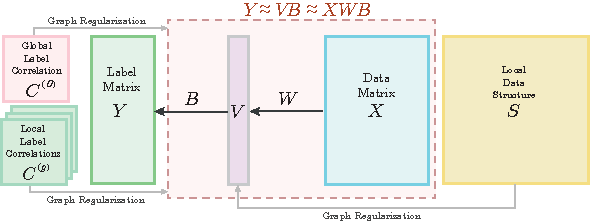
\includegraphics[width=12cm,height=5cm]{../figures/Fig1_2.pdf}
	\caption{شمای کلی روش پیشنهادی \lr{(MLFS-GLOCAL)}}
	\label{fig:1}
\end{figure}

\section{مقدمه} \label{sec31}

در این فصل، انتخاب ویژگی چندبرچسبه با استفاده از همبستگی سراسری و محلی برچسب‌ها )‎\lr{MLFS-GLOCAL‎}) معرفی می‌شود و از همبستگی برچسب‌های سراسری و محلی برای انتخاب ویژگی‌های مرتبط و غیرتکراری استفاده می‌کند. موفقیت مدل ارائه شده به چهار عامل اصلی بستگی دارد:
(1) برای ارائه یک بازنمایی برچسب-ویژگی بهینه‌تر، ساختار رتبه‌پایین را از ماتریس‌های برچسب و ویژگی استخراج می‌شود. در این فضای کاهش یافته، یک همبستگی ضمنی بین برچسب‌ها وجود دارد (بخش \ref{lowrank}‎.(
(2) جریمه‌ای\LTRfootnote{Penalty } اعمال می‌شود که همواری نگاشت محلی را در فضای نهان مشترک حفظ می‌کند (بخش \ref{LS}).
(3) با استفاده از اطلاعات همبستگی‌های سراسری و محلی برچسب، از ماتریس برچسب بصورت بهینه‌تر استفاده کرد (بخش \ref{GLOCAL}).
(4) مسئله، با ترکیب موارد فوق به یک مدل یادگیری مشترک متصل تبدیل می‌شود و از یک رویکرد کمینه‌سازی متناوب مؤثر برای بهینه‌سازی استفاده می‌کند
(بخش \ref{OPT}.(‎
شکل ‎\ref{fig:1} نمایش شماتیک از مدل ‎\lr{MLFS-GLOCAL} را ارائه می‌دهد.
\section{فضای نهان مشترک}\label{lowrank}
ماتریس ویژگی به‌صورت $\boldmath{X} \in \mathbb{R}^{n \times d}$ تعریف می‌شود و ماتریس برچسب به‌صورت $\boldmath{Y} = \{\boldmath{y}_1, {\dots}, \boldmath{y}_l\} \subseteq \{0,1\} \in \mathbb{R}^{n \times l}$ تعریف می‌شود که
${Y}_{i,j}=1$
اگر نمونه $i$-ام، برچسب $j$-ام را داشته باشد، در غیر این‌صورت  ${Y}_{ij}=0$. در مسائل داده‌های چندبرچسبه، برچسب‌ها با یکدیگر مرتبط هستند، از این رو می‌توان از رتبه‌پایین این ماتریس استفاده کرد. محتویات ماتریس خلوت $\boldmath{Y}$، دارای مقادیر دودویی و ابعاد بالا می‌باشد، بنابراین یادگیری براساس این ماتریس مشکل است. لذا اندازه ماتریس کم‌بُعد $\boldmath{Y}$ بصورت $‎‎‎k<\text{‎\lr{min}‎}(n,l)$ خواهد بود،
از این رو، ماتریس برچسب را به دو ماتریس کوچکتر به‌صورت زیر تجزیه می‌کنیم:
\begin{align}
	\boldmath{Y}\simeq\boldmath{VB}
\end{align}
که $\boldmath{V} \in \mathbb{R}^{n \times k} $ و $\boldmath{B} \in \mathbb{R}^{k \times l}$.‎


$\boldmath{V}$
ماتریس نهان برچسب‌ها است که فشرده‌تر\LTRfootnote{Compact} و از نظر معنایی انتزاعی‌تر از ماتریس برچسب‌های اصلی هستند.
$\boldmath{B}$
نشان می‌دهد که چگونه برچسب‌های اصلی با برچسب‌های نهفته مرتبط هستند. اطلاعات مهم ماتریس برچسب اصلی $\boldmath{Y}$ در ماتریس کم‌بُعد $\boldmath{V}$ کدگذاری شده است که همچنین داده‌های نامطلوب ماتریس برچسب را کاهش می‌دهد. ماتریس های $\boldmath{V}$ و $\boldmath{B}$ با به حداقل رساندن خطای بازنمایی برچسب $\lVert\boldmath{Y} - \boldmath{VB}\rVert^2_F$ بدست می‌آید. بازنمایی برچسب نهان، با $\boldmath{V}$ نشان داده شده است، یک ماتریس با ابعاد کم و با مقدار حقیقی که حاوی اطلاعات متراکم می‌باشد. بنابراین یادگیری نگاشت پیوسته از فضای ویژگی به فضای برچسب نهفته نسبتاً آسان‌تر از فضای برچسب اصلی است\cite{zhu2017multi}.
یک فرض مهم در رابطه‌ی همبستگی بین ویژگی‌ها و برچسب‌ها این می‌باشد که ویژگی‌های مشابه، برچسب‌های مشابهی دارند. در نتیجه، اطلاعات مشترک بین فضای ویژگی و فضای برچسب باید سازگار باشد. ما درنظر می‌گیریم $\boldmath{V}$ یک ماتریس مشترک بین ماتریس ویژگی و ماتریس برچسب باشد. ماتریس $\boldmath{W} \in \mathbb{R}^{d \times k}$ بروزرسانی می‌شود جهت نگاشت نمونه‌ها به فضای نهان. با کاهش خطای تابع بازنمایی ویژگی $\lVert\boldmath{V} - \boldmath{XW}\rVert^2_F$، ماتریس وزن ویژگی $\boldmath{W}$ آموخته خواهد شد و با ادغام بازنمایی برچسب و خطای بازنمایی ویژگی در یک چارچوب ماتریس نامنفی \cite{lee1999learning}، فضای نهان مشترک را از طریق تابع زیر بدست می‌آوریم:
\begin{align}
	\min_{\boldmath{V},\boldmath{B},\boldmath{W}}&\lVert\boldmath{Y}-\boldmath{V}\boldmath{B}\rVert^2_F+\lVert\boldmath{V}-\boldmath{X}\boldmath{W}\rVert^2_F,\quad{\text{\lr{s.t.}}\quad}\boldmath{{V,B,W}}\geq 0
\end{align}
\section{حفظ ساختار محلی}\label{LS}
در بسیاری از کاربرد‌های یادگیری ماشین، فضای ویژگی می‌تواند دارای ابعاد بالا همراه با نویز باشد، که استخراج اطلاعات معنی‌دار از داده‌ها را به چالش می‌کشاند. یکی از روش‌های رایج برای استخراج اطلاعات مفید، تبدیل فضای ویژگی اصلی به فضای نهان با ابعاد پایین‌تر است، جایی که ساختار زیربنایی داده‌ها را می‌توان راحت‌تر بدست ‌آورد. با این حال، بازنمایی داده‌ها در فضایی با ابعاد پایین‌تر می‌تواند منجر به از دست رفتن اطلاعات\LTRfootnote{Loss of information} شود و ممکن است روابط پیچیده بین ویژگی‌ها را به درستی نشان ندهد، از این رو از  یک منظم‌ساز گراف \cite{cai2010graph} برای ارائه یک ماتریس مناسب $\boldmath{V}$ که انسجام بین فضای ویژگی اولیه و فضای ساختار نهان را تضمین ‌کند استفاده می‌کنیم. با توجه به اصل اساسی این قاعده‌بندی، اگر دو نمونه در فضای ماتریس ویژگی $\boldmath{X}$ با یکدیگر همبستگی داشته باشند، در فضای ساختار نهان نیز هر دو نمونه $\boldmath{v}_i$ و $\boldmath{v}_j$ با یکدیگر همبستگی خواهند داشت. به‌طور خاص، ما از یک منظم‌ساز گراف برای تشویق حفظ ساختار محلی در فضای نهان استفاده می‌کنیم، و اطمینان حاصل می‌کنیم که متغیرهای نهفته به‌طور دقیق ساختار ویژگی‌های اصلی را منعکس می‌کنند. فرمول منظم‌ساز گراف را می‌توان به‌صورت زیر بیان کرد:
\begin{align} \label{eq:mfold}
	\min_{\boldmath{V}}&\frac{1}{2}\sum_{i=1}^n\sum_{j=1}^n\lVert\boldmath{v}_i-\boldmath{v}_j\rVert^2S_{i,j}\nonumber\\
	&=\frac{1}{2}\sum_{i=1}^n\sum_{j=1}^n(\boldmath{v}_i^\top\boldmath{v}_iS_{i,j}-2\boldmath{v}_i^\top\boldmath{v}_jS_{i,j}+\boldmath{v}_j^\top\boldmath{v}_jS_{i,j})\nonumber\\
	&=\frac{1}{2}\sum_{i=1}^n\sum_{j=1}^n(2\boldmath{v}_i^\top\boldmath{v}_iS_{i,j}-2\boldmath{v}_i^\top\boldmath{v}_jS_{i,j})\nonumber\\
	&=\sum_{i=1}^n\boldmath{v}_i^\top\boldmath{v}_iD_{i,i}-\sum_{i=1}^n\sum_{j=1}^n\boldmath{v}_i^\top\boldmath{v}_jS_{i,j}\nonumber\\
	&=\mathrm{Tr}(\boldmath{V}^\top\boldmath{DV})-\mathrm{Tr}(\boldmath{V}^\top\boldmath{SV})=\mathrm{Tr}(\boldmath{V}^\top \boldmath{LV}),
\end{align}
که
$\boldmath{D}$ ماتریس قطری\LTRfootnote{Diagonal} و $\boldmath{S}$ ماتریس همبستگی متقارن\LTRfootnote{Symmetric} است. $\boldmath{L} = \boldmath{D} - \boldmath{S}$ ماتریس لاپلاسین گراف می‌باشد. با ادغام عبارات فوق در مدل، تابع زیر را بدست می‌آوریم:

\begin{align}\label{eq:m-mfold}
	\min_{\boldmath{V},\boldmath{B},\boldmath{W}}&\lVert\boldmath{Y}-\boldmath{V}\boldmath{B}\rVert^2_F+\lVert\boldmath{V}-\boldmath{X}\boldmath{W}\rVert^2_F +\lambda_1{\mathrm{Tr}\boldmath{({V}^\top{LV})}}
	,\nonumber \\
	&{\text{\lr{s.t.}}}\boldmath{V},\boldmath{B},\boldmath{W}\geq 0
\end{align}
که 
$\lambda_1$
پارامتر حفظ ساختار محلی است.
\section{همبستگی برچسب سراسری و محلی}\label{GLOCAL}
برای استفاده مؤثر از اطلاعات برچسب‌ها، باید از همبستگی‌های برچسب استفاده شود. در این روش، مدل پیشنهادی را با استفاده از همبستگی برچسب مرتبه‌بالا منظم می‌کنیم. در این راستا باید به همزیستی\LTRfootnote{Coexistence} همبستگی‌های سراسری و محلی برچسب اشاره کرد. برای ترکیب هر دوی آن‌ها، منظم‌ساز خمینه برچسب‌ها را در این قسمت معرفی می‌کنیم. مفهوم منظم‌ساز خمینه سراسری برچسب‌ ‌از منظم‌ساز خمینه سطح نمونه \eqref{eq:mfold} مشتق شده است. به‌طور دقیق‌تر اگر دو برچسب دارای همبستگی بالایی باشند، خروجی‌های طبقه‌بند مربوطه آن‌ها نیز باید شباهت داشته باشند و برعکس، برچسب‌هایی که دارای همبستگی کمتری هستند باید خروجی‌های طبقه‌بند آن‌ها شباهت کمتری داشته باشند. به عبارت دیگر، همبستگی‌های برچسب منجر به خروجی‌های طبقه‌بند مشابه می‌شود. در این تحقیق از شباهت کسینوس\LTRfootnote{Cosine Similarity} برای تعیین کمیت همبستگی سراسری برچسب استفاده می‌شود $\boldmath{C} \in\mathbb{R}^{l \times l}$، که به‌صورت زیر محاسبه می‌شود: 
\begin{align}\label{eq:gloCor}	
	{{{C}_{ij}=\frac{\boldmath{y}^\top_{i}{\boldmath{y}_{j}}}{{\lVert{\boldmath{y}_i}\lVert} \lVert{\boldmath{y}_{j}}\lVert}}}
\end{align}
که
$\boldmath{y}_i$ 
, 
$\boldmath{y}_j$
به مفهوم $i$-ام و $j$-ام بردار برچسب برای همه‌ی نمونه‌ها می‌باشد.‎\\
در\eqref{eq:m-mfold}، برچسب پیش‌بینی شده برای $\boldmath{x}$ به‌صورت $f(\boldmath{x})$ است، که $f(\boldmath{x}) = \boldmath{x}\boldmath{WB}$. 
$\boldmath{f} = \{{f}_1, {\dots}, {f}_l\}$
که $\boldmath{f}_j(\boldmath{x})$ یعنی $j$-ام برچسب برای نمونه $\boldmath{x}$ پیش‌بینی شده است. در نهایت پیش‌بینی برای همه‌ی ${n}$ نمونه در ماتریس پیش‌بینی $\boldmath{F}\in\mathbb{R}^{n \times l}$ ذخیره می‌شود،‌ $\boldmath{F}= \{f({\boldmath{x}}_1),{\dots},f({\boldmath{x}}_n)\}^\top = \boldmath{XWB}$ شامل محتویات پیش‌بینی شده برای $i$-ام برچسب $\boldmath{f}_i$، اگر برچسب ${i}$-ام و ${j}$-ام شبیه باشند باید بردار پیش‌بینی شده
$\boldmath{f}_j$ و $\boldmath{f}_i$
این دو برچسب نیز شبیه باشند و برعکس. تعریف منظم‌ساز خمینه ‌سراسری برچسب شبیه تعریف منظم‌ساز خمینه نمونه \eqref{eq:mfold} است و به‌صورت زیر تعریف می‌شود:
\begin{align}\label{eq:glomfold}
	\min_{\boldmath{F}}&\frac{1}{2}\sum_{i=1}^l\sum_{j=1}^l\lVert\boldmath{f}_i-\boldmath{f}_j\rVert^2C_{i,j}=\nonumber\\
	&\mathrm{Tr}(\boldmath{FA}\boldmath{F}^\top)-\mathrm{Tr}(\boldmath{FC}\boldmath{F}^\top)=\mathrm{Tr}(\boldmath{FP}\boldmath{F}^\top),\nonumber\\
\end{align}
$\boldmath{A}$ ماتریس قطری و به‌صورت ${A}_{ii}=\sum_{j=1}^l {C}_{ij}$ تعریف می‌شود. 
با کمینه‌سازی کردن \eqref{eq:glomfold}، خطای $\lVert\boldmath{f}_i-\boldmath{f}_j\rVert^2 $ کم خواهد بود. منظم‌ساز خمینه در \eqref{eq:glomfold} به‌صورت $\mathrm{Tr}(\boldmath{FPF}^\top)$، که $\boldmath{P} = \boldmath{A}-\boldmath{C}$ ماتریس لاپلاسین ‌است. $\boldmath{F}=\boldmath{XWB}$ برچسب‌های پیش‌بینی شده برای ویژگی‌ها می‌باشد. از آنجایی که همبستگی‌های برچسب می‌تواند در نواحی مختلف محلی متفاوت باشد، برای استخراج این همبستگی‌ها از منظم‌ساز خمینه محلی استفاده می‌کنیم. فرض می‌کنیم که مجموعه‌داده\LTRfootnote{Dataset} $\boldmath{X}$ به ${g}$ گروه $\{\boldmath{X}_1,{\dots},\boldmath{X}_g\}$ تقسیم می‌شود، ماتریس $\boldmath{X}_m \in \mathbb{R}^{n_m \times d}$ نمونه دارد. با استفاده از خوشه‌بندی، مانند شبکه‌ها\LTRfootnote{Networks} و مسیرهای ژنی\LTRfootnote{Pathways} \cite{chuang2007network,subramanian2005gene} در کاربردهای بیوانفورماتیک\LTRfootnote{Bioinformatics}، امکان دستیابی به این پارتیشن‌بندی وجود دارد. فرض  $\boldmath{C}_m \in \mathbb{R}^{{l} \times {l}}$ ماتریس همبستگی برچسب محلی یک گروه ${m}$ است. و $\boldmath{Y}_m$ زیر ماتریس برچسب در $\boldmath{Y}$ متناظر با $\boldmath{X}_m$ است. مانند \eqref{eq:gloCor}، ما همبستگی‌های برچسب محلی را به‌صورت زیر محاسبه می‌کنیم:

\begin{align}\label{eq:llc}	
	{{{C}^{(m)}_{i,j}}=
		\frac
		{{\boldmath{y}^{(m)}_{i}}^\top\boldmath{y}^{(m)}_{j}}
		{{\lVert{\boldmath{y}^{(m)}_{i}}\lVert}\lVert{\boldmath{y}^{(m)}_{j}}\lVert}}, \; m \in  \{1,{\dots},{g}\}
\end{align}
مشابه همبستگی برچسب سراسری \eqref{eq:glomfold}، اگر دو برچسب با همدیگر همبستگی داشته باشند باید بردار ‎‎پیش‌بینی شده‎ طبقه‌بند نیز شبیه باشند:
\begin{align}\label{eq:loclmfold}
	\min_{\boldmath{F}}&\sum_{m=1}^{g}\frac{n_m}{n}\sum_{i=1}^{l}\sum_{j=1}^{l} \lVert{\boldmath{f}^{(m)}_i}-{\boldmath{f}^{(m)}_j}\rVert^2 {C^{(m)}_{i,j}}\nonumber \\
	&=\sum_{m=1}^{g} \frac{n_m}{n}[\mathrm{Tr}(\boldmath{F}_m\boldmath{A}_m\boldmath{F}_m^\top) - \mathrm{Tr}(\boldmath{F}_m \boldmath{C}_m \boldmath{F}_m^\top)]\nonumber \\
	&= \sum_{m=1}^{g}\frac{n_m}{n}\mathrm{Tr}(\boldmath{F}_m \boldmath{P}_m \boldmath{F}_m^\top)
\end{align}
که $\boldmath{F}_m = \boldmath{X}_m\boldmath{WB}$ ماتریس خروجی طبقه‌بند برای گروه $m$ است و $\boldmath{P}_m$ ماتریس لاپلاسین $\boldmath{C}_m$ است. برای پوشش عدم تعادل\LTRfootnote{Imbalance} خوشه، منظم‌ساز همبستگی محلی برچسب را با ضریب ${n_m}/{n}$  نرمال می‌کنیم.
پس از افزودن منظم‌سازهای خمینه سراسری \eqref{eq:glomfold} و محلی  \eqref{eq:loclmfold} به تابع \eqref{eq:m-mfold}، فرمول زیر بدست می‌آید:
\begin{align}
	&\min_{\boldmath{V},\boldmath{B},\boldmath{W}}\lVert\boldmath{Y}-\boldmath{V}\boldmath{B}\rVert^2_F+\lVert\boldmath{V}-\boldmath{X}\boldmath{W}\rVert^2_F+\lambda_1{\mathrm{Tr}\boldmath{({V}^\top{LV})}}
	\nonumber \\&+\lambda_2[\mathrm{Tr}(\boldmath{FP}\boldmath{F}^\top) 
	+ \sum_{m=1}^{g}\frac{n_m}{n}\mathrm{Tr}(\boldmath{F}_m\boldmath{P}_m\boldmath{F}^\top_m) ],
	\quad{\text{\lr{s.t.}}\quad}\boldmath{V},\boldmath{B},\boldmath{W}\geq 0 
\end{align}
که $\lambda_2$ نشان دهنده تأثیر همبستگی برچسب سراسری و محلی برای تابع هدف است. در نهایت، تابع ما از نُرم $\ell_{2,1} $، که برای انتخاب ویژگی است استفاده می‌کند. در نتیجه تابع نهایی به‌صورت زیر تنظیم می‌شود: 
\begin{align}\label{eq:BeOpt}
	&\min_{\boldmath{V},\boldmath{B},\boldmath{W}}\lVert\boldmath{Y}-\boldmath{V}\boldmath{B}\rVert^2_F+\lVert\boldmath{V}-\boldmath{X}\boldmath{W}\rVert^2_F+\lambda_1{\mathrm{Tr}\boldmath{({V}^\top{LV})}} \nonumber \\ 
	& +\lambda_2[\mathrm{Tr}(\boldmath{FP}\boldmath{F}^\top)+\sum_{m=1}^{g}\frac{n_m}{n}\mathrm{Tr}(\boldmath{F}_m\boldmath{P}_m\boldmath{F}^\top_m) ]+ \lambda_3\lVert\boldmath{W}\rVert_{2,1},\nonumber \\ &{\text{\lr{s.t.}}}\boldmath{V},\boldmath{B},\boldmath{W}\geq 0 \nonumber \\
\end{align}
با استفاده از نُرم $\ell_{2,1} $ بر روی سطر ماتریس $\boldmath{W}$ خلوتی اعمال می‌کنیم و منظم‌ساز خلوتی تابع هدف نیز توسط پارامتر $\lambda_3$ کنترل می‌شود.

\section{بهینه‌سازی}\label{OPT} 
تابع \eqref{eq:BeOpt} شامل عبارت منظم‌ساز نُرم $\ell_{2,1} $ است. از آنجا که این تابع هموار نیست، همچنین وقتی متغیرهای $\boldmath{V}$، $\boldmath{B}$ و $\boldmath{W}$ به‌صورت ترکیبی درنظر گرفته می‌شوند، غیرمحدب\LTRfootnote{Non-convex} می‌شود. به‌عبارت دیگر، ماتریس هسین\LTRfootnote{Hessian matrix} که از مشتقات جزئی تابع هدف در درجه‌دوم بدست می‌آید، ماتریسی نیست که نیمه مثبت معین\LTRfootnote{Semi-definite} باشد. بنابراین، تابع هدف باید به گونه‌ای بهینه‌سازی شود که در هر مرحله از الگوریتم با ثابت نگه‌داشتن سه متغیر و به‌روزرسانی متغیر باقیمانده به‌صورت محدب\LTRfootnote{Convex} باشد. عبارت $\lVert\boldmath{W}\rVert_{2,1}$ با استفاده از $\mathrm{Tr} (\boldmath{W^\top DW})$ به شکلی دیگر خفیف می‌شود، که در این حالت $\boldmath{D}$ یک ماتریس قطری است \cite{hu2020multi}. الگوریتم مبتنی بر تکراری ویژگی‌های بروزرسانی در دسترس است. درایه $\boldmath{D}$ به شکل $D_{ii} = 1/(\lVert \boldmath{w}_i\lVert+\epsilon),(\epsilon\leftarrow0)$ است.
که $\epsilon$ برای جلوگیری از اختلال در محاسبات مسئله بکار می‌رود. به عبارت دیگر، تابع هدف \eqref{eq:BeOpt} می‌تواند به‌صورت زیر بازنویسی شود:
\begin{align}\label{eq:1stopt}
	&\min_{\boldmath{V},\boldmath{B},\boldmath{W}}\lVert\boldmath{Y}-\boldmath{V}\boldmath{B}\rVert^2_F+\lVert\boldmath{V}-\boldmath{X}\boldmath{W}\rVert^2_F+\lambda_1{\mathrm{Tr}\boldmath{({V}^\top{LV})}}\nonumber \\
	&+\lambda_2[\mathrm{Tr}(\boldmath{FP}\boldmath{F}^\top)+\sum_{m=1}^{g}\frac{n_m}{n}\mathrm{Tr}(\boldmath{F}_m\boldmath{P}_m\boldmath{F}^\top_m) ]+ \lambda_3(\boldmath{W}^\top \boldmath{DW}),\nonumber\\
	& {\text{\lr{s.t.}}}\boldmath{V},\boldmath{B},\boldmath{W}\geq 0 
\end{align}
ما برای افزودن محدودیت نامنفی در تابع، ضرایب لاگرانژی\LTRfootnote{Lagrangian multipliers} را معرفی می‌کنیم. 
$\boldmath{\Phi}$، $\boldmath{\Psi}$
و $\boldmath{\Omega}$ برای محدود کردن $\boldmath{V}$، $\boldmath{B}$ و $\boldmath{W}$ به ترتیب، جایی که $\boldmath{\Phi} \in\mathbb {R}^{n \times k}$, $\boldmath{\Psi} \in\mathbb{R}^{k \times l}$, $\boldmath{\Omega} \in\mathbb{R}^ {d \times k}$، در نتیجه، تابع \eqref{eq:1stopt} معادل زیر است:
\begin{align}\label{eq:2ndopt}
	&\min_{\boldmath{V}, \boldmath{B}, \boldmath{W}}\lVert\boldmath{Y}-\boldmath{V}\boldmath{B}\lVert^2_F + \lVert\boldmath{V}-\boldmath{X}\boldmath{W}\lVert^2_F+ \lambda_1\mathrm{Tr}(\boldmath{V}^\top \boldmath{LV})\nonumber \\
	&+\lambda_2[\mathrm{Tr}(\boldmath{F}\boldmath{P}\boldmath{F}^\top) + \sum_{m=1}^{g}\frac{n_m}{n}\mathrm{Tr}(\boldmath{F}_m\boldmath{P}_m\boldmath{F}_m^\top)]\nonumber\\
	&+\lambda_3\mathrm{Tr}(\boldmath{W}^\top \boldmath{D}\boldmath{W})- \mathrm{Tr}(\boldmath{\Phi}\boldmath{V}^\top)    -\mathrm{Tr}(\boldmath{\Psi}\boldmath{B}^\top)-\mathrm{Tr}(\boldmath{\Omega}\boldmath{W}^\top)\nonumber\\
\end{align}
با توجه به ماتریس $\boldmath{A}$, $\lVert \boldmath{A} \lVert^2_F = \mathrm{Tr}(\boldmath{A}^\top \boldmath{A})$. بنابراین، تابع \eqref{eq:2ndopt} تبدیل می‌شود:

\begin{align}\label{eq:3rdopt}
	C =  &\mathrm{Tr}[(\boldmath{Y} - \boldmath{V}\boldmath{B})^\top (\boldmath{Y} - \boldmath{V}\boldmath{B})]+ \mathrm{Tr}[(\boldmath{V}-\boldmath{X}\boldmath{W})^\top(\boldmath{V} - \boldmath{X}\boldmath{W})]\nonumber\\
	&+\lambda_1\mathrm{Tr}(\boldmath{V}^\top \boldmath{LV})+\lambda_2[\mathrm{Tr}(\boldmath{F}\boldmath{P}\boldmath{F}^\top)+ \sum_{m=1}^{g}\frac{n_m}{n}\mathrm{Tr}(\boldmath{F}_m\boldmath{P}_m\boldmath{F}_m^\top)]\nonumber\\
	&+ 2 \lambda_3\mathrm{Tr}(\boldmath{W}^\top \boldmath{D}\boldmath{W})- \mathrm{Tr}(\boldmath{\Phi}\boldmath{V}^\top) -\mathrm{Tr}(\boldmath{\Psi}\boldmath{B}^\top) -\mathrm{Tr}(\boldmath{\Omega}\boldmath{W}^\top)
\end{align}
که $\boldmath{F}=\boldmath{XWB}$ و $‎\boldmath{F}_m=\boldmath{X}_m\boldmath{WB}‎$, $\forall m \{1,{\dots},{g}\}$. مشتقات جزئی تابع \eqref{eq:3rdopt} با توجه به متغیرهای $‎\boldmath{V}$, $ \boldmath{B}$ و $\boldmath{W}$ عبارتند از:
\begin{align}\label{eq:derW}
	&\frac{\partial C}{\partial\boldmath{W}} = {-\boldmath{X}^\top \boldmath{V} + \boldmath{X}^\top \boldmath{XW} + \lambda_2[\boldmath{X}^\top \boldmath{XWBPB}^\top}\nonumber\\
	&+ \sum_{m=1}^{g}\frac{n_m}{n} \boldmath{X}^\top_m \boldmath{X}_m\boldmath{WBP}_m\boldmath{B}^\top]+ 2\lambda_3\boldmath{DW}-\boldmath{\Omega}
\end{align}

\begin{align}\label{eq:derB}
	\frac{\partial C}{\partial \boldmath{B}} = &{-\boldmath{V}^\top \boldmath{Y} + \boldmath{V}^\top \boldmath{VB} + \lambda_2[\boldmath{W}^\top \boldmath{X}^\top \boldmath{XWBP}} \nonumber \\
	& \quad\quad+ \sum_{m=1}^{n} \frac{n_m}{n}\boldmath{W}^\top \boldmath{X}^\top_m \boldmath{X}_m\boldmath{WBP}_m] - \boldmath{\Phi}
\end{align}	

\begin{align}\label{eq:derV}
	\frac{\partial C}{\partial \boldmath{V}} = {\boldmath{V} - 2\boldmath{XW} - 2\boldmath{YB}^\top + \boldmath{VBB}^\top + \lambda_1\boldmath{LV} -\boldmath{\Psi}}.
\end{align}

با قرار دادن مشتقات جزئی \eqref{eq:derW}، \eqref{eq:derB} و \eqref{eq:derV} برابر با صفر، می‌توانیم نقاط بهینه\LTRfootnote{Optimal points} تابع را پیدا کنیم. با توجه به شرایط\LTRfootnote{Conditions} 
\lr{Karush-Kuhn-Tucker}، $\boldmath{W}\odot\boldmath{\Omega}=\boldmath{0}$، $\boldmath{B}\odot\boldmath{\Phi}=\boldmath{0}$ و $\boldmath{V}\odot\boldmath{\Psi}=\boldmath{0}$ را تنظیم می‌کنیم. با حل این معادلات، توابع به‌روزرسانی زیر را برای $\boldmath{W}$، $\boldmath{B}$ و $\boldmath{V}$ بدست می‌آوریم:‎\\
\begin{align*}
	&\boldmath{\Omega}_{SGC}=\boldmath{X}^\top \boldmath{XWBCB}^\top & \\
	&\boldmath{\Omega}_{DGC}=\boldmath{X}^\top \boldmath{XWBAB}^\top & \\
	&\boldmath{\Omega}_{SLC}=\frac{n_m}{n}\boldmath{X}^\top_m \boldmath{X}_m\boldmath{WBC}_m\boldmath{B}^\top & \\
	&\boldmath{\Omega}_{DLC}=\frac{n_m}{n}\boldmath{X}^\top_m\boldmath{X}_m\boldmath{WBA}_m\boldmath{B}^\top & \\
\end{align*}
\begin{align}\label{eq:updW}
	\boldmath{W} \leftarrow \boldmath{W} \odot \frac{\boldmath{X}^\top \boldmath{V} + \lambda_2[\boldmath{\Omega}_{SGC}+ \sum_{m=1}^{g}\boldmath{\Omega}_{SLC}]}
	{\boldmath{X}^\top \boldmath{XW} + \lambda_2[\boldmath{\Omega}_{DGC} +\sum_{m=1}^{g}\boldmath{\Omega}_{DLC}]+\lambda_3\boldmath{DW}}
\end{align}
\begin{align*}
	&\boldmath{\Xi}_{SLC}=\frac{n_m}{n}\boldmath{W}^\top \boldmath{X}^\top_m \boldmath{X}_m\boldmath{WBC}_m & \\
	&\boldmath{\Xi}_{DLC}=\frac{n_m}{n}\boldmath{W}^\top \boldmath{X}^\top_m \boldmath{X}_m\boldmath{WBA}_m & \\
	&\boldmath{\Xi}_{SGC}=\boldmath{W}^\top \boldmath{X}^\top \boldmath{XWBC} & \\
	&\boldmath{\Xi}_{DGC}=\boldmath{W}^\top \boldmath{X}^\top \boldmath{XWBA} & \\
\end{align*}
\begin{align}\label{eq:updB}
	\boldmath{B} \leftarrow \boldmath{B}\odot \frac{\boldmath{V}^\top \boldmath{Y} +\lambda_2[\boldmath{\Xi}_{SGC} +\sum_{m=1}^{g} \boldmath{\Xi}_{SLC} ]}{\boldmath{V}^\top \boldmath{VB} + \lambda_2[\boldmath{\Xi}_{DGC} +\sum_{m=1}^{g} \boldmath{\Xi}_{DLC}] }
\end{align}
\begin{align}\label{eq:updV}
	\boldmath{V} \leftarrow \boldmath{V} \odot \frac{\boldmath{XW} + \boldmath{YB}^\top + \lambda_1 \boldmath{SV}}{\boldmath{V} +\boldmath{VBB}^\top + \lambda_1 \boldmath{DV}}
\end{align}

\lr{MLFS-GLOCAL} تمام ویژگی‌ها را با استفاده از $\lVert \boldmath{w}_i\lVert_2, (i=1,{\dots},{d})$ به ترتیب نزولی رتبه‌بندی می‌شود و به ما امکان می‌دهد تا ویژگی‌های با بالاترین امتیاز را بدست‌ آوریم. الگوریتم \ref{alg:algorithm} مدل \lr{MLFS-GLOCAL} را به‌صورت جزئیات تشریح می‌کند.

\lr{
	\begin{algorithm}[tb]	
		\setstretch{1} 
		\caption{Multi-label Feature Selection with Global and Local label correlation\\ {(MLFS-GLOCAL)}}
		\begin{flushleft}
			\textbf{Input}: Feature matrix $\boldmath{X}$$\in$$\mathbb{R}^ {n \times d}$ and Label matrix
			$\boldmath{Y}$$\in$$\mathbb{R}^{n \times c}$, Regularization parameters $\lambda_1,\lambda_2$, and $\lambda_3$, and latent factor $k$;\\
			\textbf{Output}: Feature score $s_i=\lVert\boldmath{w}_i\rVert, \forall i\in\{1,2,{\dots},d\}$.
		\end{flushleft}
		\begin{algorithmic}[1] %[1] enables line numbers
			\STATE \textbf{Initialize} $\boldmath{V},\boldmath{W},\boldmath{B}$ randomly; $t=0;$
			\WHILE{$t <$ MaxIteration}
			\STATE Update $D_{ii}\leftarrow\frac{1}{\lVert\boldmath{w}_i\rVert+\epsilon}$;
			\STATE  Update $\boldmath{W}$ by \eqref{eq:updW};
			\STATE Update $\boldmath{B}$ by \eqref{eq:updB};
			\STATE Update ${\boldmath{V}}$ by \eqref{eq:updV};
			\STATE $t = t + 1$;
			%\STATE $\textbf{Until}$ Convergence;
			\ENDWHILE
			\STATE $\textbf{Return}$ $\boldmath{W}$;
			\STATE Evaluate the feature score by $s_i=\lVert\boldmath{w}_i\rVert$.
		\end{algorithmic}
		\label{alg:algorithm}
	\end{algorithm}
}
	\titleformat{\chapter}[display]
{\normalfont\Large\BNazboldEGT\centering}
{\vspace*{8cm}{‎\textbf{فصل چهارم} }}{5pt}{\Large}
\chapter{\textbf{آزمایشات}}\label{sec4}
\thispagestyle{empty}
\newpage

\begin{table}
	\centering
	\small
	\caption{جزئیات مجموعه‌داده‌های دنیای واقعی}
	\setLTRtable
	\begin{tabular}{lcccccc}
		\hline
		مجموعه‌داده & \#نمونه & \#ویژگی & \#برچسب\\
		\hline
		\lr{Arts}       & 5000 & 462 & 26 \\
		\lr{Business}   & 5000 & 438 & 30 \\
		\lr{Computers}  & 5000 & 681 & 33 \\
		\lr{corel5k}    & 5000 & 499 & 374 \\
		\lr{Education}  & 5000 & 550 & 33 \\
		\lr{Entertainment} & 5000 & 640 & 21 \\
		\lr{Health}     & 5000 & 612 & 32 \\
		\lr{Recreation} & 5000 & 606 & 22 \\
		\lr{Reference}  & 5000 & 793 & 33 \\
		\lr{Science}    & 5000 & 743 & 40 \\
		\lr{Social}     & 5000 & 1047 & 39 \\
		\lr{Society}    & 5000 & 636 & 27 \\
		\hline
	\end{tabular}
	\label{tab:datasets}
\end{table}
این بخش یک ارزیابی جامع برای مدل ‎\lr{MLFS-GLOCAL}‎ بر روی 12 مجموعه‌داده چندبرچسبه واقعی با استفاده از شش معیار\LTRfootnote{Metric}} ارزیابی متنوع انجام می‌دهد. همچنین مدل پیشنهادی با نُه روش شناخته‌شده و پیشرفته انتخاب ویژگی مقایسه شده است.‎
\section{مجموعه‌داده‌ها}
در بخش آزمایشات، از ۱۲ مجموعه‌داده از کتابخانه \lr{Mulan} برای طبقه‌بندی متن و تصاویر چندبرچسبه استفاده شده است. مجموعه‌داده‌های چندبرچسبه یاهو\LTRfootnote{Yahoo} به مجموعه‌ای از چندین مجموعه‌داده اشاره دارد که برای طبقه‌بندی مسائل چندبرچسبه استفاده می‌شوند. این‌ داده‌ها، توسط آزمایشگاه‌های یاهو منتشر شدند و شامل تعداد زیادی اسناد متنی است که به چندین برچسب مرتبط می‌باشند. هر مجموعه‌داده شامل مجموعه آموزش\LTRfootnote{Train} و مجموعه آزمایش\LTRfootnote{Test} است که هرکدام به ترتیب شامل ۲۰۰۰ و ۳۰۰۰ سند\LTRfootnote{Document} هستند \cite{doquire2013mutual}. 
مجموعه‌داده چندبرچسبه \lr{Corel5k} مجموعه‌ایی از تصاویر است که برای طبقه‌بندی چندبرچسبه استفاده می‌شود. این مجموعه شامل ۵۰۰۰ تصویر از ۳۷۴ دسته‌بندی مختلف است و هر تصویر دارای چندین برچسب است.
مجموعه‌داده‌های یاهو و \lr{Corel5k} به‌طور گسترده در تحقیقات جهت توسعه و ارزیابی الگوریتم‌های طبقه‌بندی چندبرچسبه استفاده شده‌‌اند. جدول \ref{tab:datasets} ویژگی‌های هر مجموعه‌داده مرجع را توصیف می‌شود.
\section{معیارهای ارزیابی}

برای ارزیابی عملکرد روش‌های رقیب، از \lr{Multi-Label kNN (ML-kNN)} \cite{zhang2007ml} برای طبقه‌بندی استفاده می‌شود. \lr{ML-kNN} به دلیل تفسیرپذیری و سادگی به‌عنوان یک الگوریتم متداول برای طبقه‌بندی در رویکردهای انتخاب ویژگی چندبرچسبه استفاده می‌شود \cite{liu2018online,zhang2019manifold,jian2016multi,hu2020multi}. ما $\text{\lr{k}}= 10$ را برای تعداد همسایه‌ها\LTRfootnote{Neighbours} قرار دادیم، علاوه بر این، از شش معیار ارزیابی متداول استفاده می‌کنیم که شامل \lr{Micro-F1}، \lr{Macro-F1}، \lr{Average Precision}، \lr{Ranking Loss}، \lr{Hamming Loss} و \lr{Coverage Error} هستند. تعاریف این معیارها به شرح زیر است:

\begin{itemize}
	
	\item	\lr{Micro-F1 , Macro-F1} :
	
	هر دو براساس معیار اندازه‌گیری ‎ \lr{ F-measure}‎.هستند معیار ارزیابی مستقیماً از میانگین‌‌‌ \lr{F-measure}‎ استفاده می‌شود برای رتبه‌بندی دقت پیش‌بینی‌ها که توسط طبقه‌بند برچسب تولید شده‌اند.
	\begin{align}
		{Micro-F1} = \frac{\sum_{i=1}^{l} 2 TP^i}{\sum_{i=1}^{l}(2 TP^i + FP^i + FN^i)},
	\end{align}
	\begin{align}
		{Macro-F1} = \sum_{i=1}^{l} \frac{2 TP^i}{2 TP^i + FP^i + FN^i},
	\end{align}
	که در آن \lr{TP}‎، ‎\lr{FP}‎ و ‎\lr{ FN}‎به ترتیب مثبت صحیح\LTRfootnote{True positive}، مثبت کاذب\LTRfootnote{False positive} و منفی کاذب\LTRfootnote{False negative} هستند.
	
	\item \lr{Average Precision}:
	
	
	این معیار مشخص می‌کند درصد برچسب‌هایی که بیشتر از یک برچسب‌خاص مرتبط هستند:
	
	\begin{align}
		{AP(D)} = \frac{1}{n} \sum_{i=1}^{n} \frac{1}{1^\top_m y_i} \sum_{l:y^l_i}^{}\frac{prec_i(l)}{rank_i(l)},
	\end{align}
	که‎
	$prec_i(l)=\sum_{l:y^l_i=1}^{} \delta(rank_i(l) \geq rank_i(l^\prime))$ و $AP(D) \in \lceil 0,1 \rceil $.
	
	\item	\lr{Ranking Loss}:
	در این معیار، نسبت دو برچسبی که به‌ترتیب معکوس یا مهم‌تر از برچسب‌های مرتبط درنظر گرفته شده است.
	\begin{align}
		{RL(D)} = \frac{1}{n} \sum_{i=1}^{n} \frac{1}{1^\top_m y_i 1^\top_m \overline{y_i}} \sum_{l:y^l_i=1}^{}\sum_{l^\prime:y^l_i=0}^{}(\delta(rank_i(l) \geq rank_i(l^\prime))),
	\end{align}
	%$RL(D)\in [0, 1]$
	که 
	$\overline{y_i}$ 
	مکمل
	$y_i$ در $\boldmath{Y}$ و $‎RL(D) \in [0, 1]$
	می‌باشد.
	\item	\lr{Hamming Loss}:
	در \lr{HL}‎ درصد برچسب‌هایی را تعیین می‌کند که به اشتباه برچسب‌ گذاری شده‌اند.
	\begin{align}
		{HL(D)} = \frac{1}{n} \sum_{i=1}^{n} \frac{1}{m} \lVert h(x_i) \Delta y_i \lVert_1,
	\end{align}
	نماد $\Delta$ برای نمایش تفاضل همسان بین دو مجموعه استفاده می‌شود و مجموعه‌ای از مقادیر است که اختصاصاً در یکی از دو مجموعه ظاهر می‌شود.
	
	\item	\lr{Coverage Error}:
	در این معیار خطای پوشش یک معیار ارزیابی است که تعداد مراحل یا پیش‌بینی‌های مورد نیاز برای پوشش تمام برچسب‌های مثبت مرتبط با نمونه‌ها را با پایین آمدن رتبه‌بندی برچسب‌های پیش‌بینی‌شده اندازه‌گیری می‌شود.
	\begin{align}
		{CV(D)} = \frac{1}{n} \sum_{i=1}^{n} \arg \max_{l:y^l_i=1}rank_i(l)-1,
	\end{align}
	
	مقدار کوچک در ‎\lr{Ranking Loss} ,‎\lr{Hamming Loss} ,‎\lr{Coverage Error}‎‎‎ بیانگر عملکرد بهتر مدل می‌باشد و مقدار صفر ایده‌آل است، درحالی که در معیارهای
	\lr{Micro-F1} ,‎\lr{Macro-F1} ‎, \lr{Average Precision} ‎‎مقادیر بالا بیانگر عملکرد بهتر الگوریتم می‌باشد و مقدار یک مقدار ایده‌آل می‌باشد.
\end{itemize}
\section{روش‌های مقایسه‌شده}

در این بخش، روش پیشنهادی با روش‌های جدید انتخاب ویژگی در داده‌های چندبرچسبه مقایسه شده‌ است که در زیر توضیحات مختصری درباره‌ی هرکدام از روش‌ها داده شده است.


\begin{itemize}
	
	\item \lr{MDMR} \cite{lin2015multi}: یک روش ‌انتخاب ویژگی مبتنی بر تئوری‌اطلاعات است که ویژگی‌ها را با حداکثر کردن وابستگی و به حداقل رساندن افزونگی همزمان انتخاب می‌کند.
	
	\item \lr{SCLS} \cite{lee2017scls}: یکی دیگر از الگوریتم های انتخاب ویژگی است که از تئوری‌اطلاعات استفاده می‌کند و ارتباط شرطی را با استفاده از یک معیار ارزیابی ارتباط مقیاس‌پذیر ارزیابی می‌کند.
	
	\item \lr{LRFS} \cite{zhang2019distinguishing}: مبتنی بر افزونگی برچسب‌ها می‌باشد. در این روش از اطلاعات متقابل شرطی استفاده می‌شود برای ایجاد یک عبارت جدید ویژگی مرتبط جهت ارزیابی اطلاعات ویژگی‌ها.
	
	\item \lr{MIFS} \cite{jian2016multi}: یک روش شناخته شده \lr{MLFS} است که از معنای نهان ماتریس چندبرچسبه برای انتخاب مهم‌ترین ویژگی‌ها استفاده می‌کند.
	
	\item \lr{CMFS} \cite{braytee2017multi}: روشی برای مطالعه اطلاعات ساختار‌یافته است که بر همبستگی‌های ویژگی‌ها و برچسب تکیه دارد. 
	
	\item \lr{SCMFS} \cite{hu2020multi}: از تجزیه ماتریس نامنفی جفت شده برای ایجاد مدل مشترک استفاده می‌کند.
	
	\item \lr{SSFS} \cite{gao2021multilabel}: یک عبارت مشترک ساختار نهان (\lr{LSS}) را پیشنهاد کرد که هر دو ویژگی نهان و ساختار برچسب را به اشتراک گذاشته و حفظ می‌کند.
	
	\item \lr{MRDM} \cite{huang2021multi}: از \lr{HSIC} به‌عنوان یک معیار جهت افزایش رابطه بین خمینه تعبیه شده و برچسب‌های کلاس استفاده می‌شود.
	
	\item \lr{NMDG} \cite{zhang2022non}: از ماتریس لاپلاسین گراف پویا ساخته شده توسط شبه‌برچسب در فرآیند انتخاب ویژگی استفاده می‌کند.
	
\end{itemize}

%\begin{table}
%	\centering
%	\small
%%	\renewcommand{\arraystretch}{1}
%	\caption{جزئیات مجموعه‌داده‌‌های دنیای واقعی}
%
%		\begin{tabular}{rcccccc}
	%			\hline
	%‎\multicolumn{1}{1}{‎\#مجموعه‌داده} &  ‎\multicolumn{1}{1}‎{\#نمونه‌ها} & \multicolumn{1}{1}{\#ویژگی} & 	\multicolumn{1}{1}{\#برچسب}\\ 	\hline
	%
	%			\lr{Arts}      &  5000 &   462&   26  \\
	%			\lr{Business}  &  5000 &   438&   30  \\
	%			\lr{Computers} &  5000 &   681&   33  \\
	%			\lr{corel5k}   &  5000 &  499 &  374  \\
	%			\lr{Education} &  5000 &  550 &  33   \\
	%			\lr{Entertainment}&5000&  640 &  21   \\
	%			\lr{Health}    &  5000 &  612 &  32   \\
	%			\lr{Recreation}&  5000 &  606 &  22   \\
	%			\lr{Reference} &  5000 &  793 &  33   \\
	%			\lr{Science}   &  5000 &  743 &  40   \\
	%			\lr{Social}    &  5000 &  1047&  39   \\
	%			\lr{Society}   &  5000 &  636 &  27   \\
	%			\hline
	%		\end{tabular}
%		\label{tab:datasets}
%%	\renewcommand{\arraystretch}{}
%\end{table}

\section{نتایج آزمایشات}
در بخش نتایج آزمایشات، ما $\%$20 از ویژگی‌های برتر را برای تعیین میانگین عملکرد برای هر روش انتخاب کردیم. جداول \ref{tab:MicT} تا \ref{tab:CVET} نتایج این آزمایش‌ها را بر روی شش معیار ارزیابی مختلف نشان می‌دهند. بهترین نتایج برای هر مجموعه‌داده با فونت ضخیم نشان داده می‌شود، جایی که هر چه مقادیر بالاتر باشد، عملکرد طبقه‌بند بهتر است. برای ارائه یک ارزیابی پایدار‌‌ از عملکرد مدل‌ها، هر روش 10 بار اجرا شده‌ است و میانگین نتایج برای همه‌ی مجموعه‌داده‌ها گزارش می‌شود. نتایج نشان می‌دهد که در اکثر مجموعه‌داده‌ها، مدل پیشنهادی بهترین نتایج را کسب کرده‌است. علاوه بر این، بهترین 
امتیاز‎\lr{Micro-F1} ‎ توسط ‎\lr{MLFS-GLOCAL}‎ بدست آمد که در مجموعه‌داده‌های ‎\lr{Arts}‎، ‎\lr{Corel5k}‎، ‎\lr{Entertainment}‎، ‎\lr{Health}‎، ‎\lr{Recreation}‎ و ‎\lr{Social}‎ برتری قابل توجهی نسبت به روش دوم‌برتر داشت است. جداول نشان می‌دهند که مدل پیشنهادی در 67 مورد از 72 مورد مقایسه، اول و در بقیه‌ موارد در رتبه‌دوم قرار دارد.‌ نتایج تأیید می‌کنند که روش ما می‌تواند برای طیف گسترده‌ای از مجموعه‌های داده، برخلاف روش‌های دیگر، اعمال شود. به‌طور متوسط، ما بهبودهای قابل توجهی را در مقادیر این معیارها مشاهده کردیم، با 0367.0 برای 
\lr{Micro-F1}،
0157.0 برای
\lr{Macro-F1}،
0443.0 برای 
‎\lr{Average Precision}‎،
222.0 برای
‎\lr{Coverage Error}‎،
{0014.0} برای
‎\lr{Hamming Loss}‎ و
{0011.0} برای
\lr{Ranking Loss}‎.
\begin{table}
	\centering
	\renewcommand{\arraystretch}{1.3}
	\caption{ارزیابی مدل بر اساس معیار \lr{Micro-F1}}
	\scriptsize
	\setlength{\tabcolsep}{2.4pt}
	\setLTRtable
	\begin{tabular}{l>{\arraybackslash$}<{$}cccccccccc}
		\hline			\textbf{مجموعه‌داده}      & \textbf{SSFS} & \textbf{SCMFS} & \textbf{MIFS} & \textbf{CMFS} & \textbf{MRDM} & \textbf{NMDG} & \textbf{SCLS} & \textbf{LRFS} & \textbf{MDMR} & \textbf{MLFS-GLOCAL} \\
		\hline
		{Arts}          & 0.2263        & \persianunderline{0.2674}   & 0.1655        & 0.1753        & 0.2496        & 0.1714           & 0.1258        & 0.0601        & 0.1418        & \textbf{0.3230}    \\
		{Business}      & 0.6816        & \persianunderline{0.6927}   & 0.6846        & 0.6786        & 0.6892        & 0.6728           & 0.6760        & 0.6698        & 0.6704        & \textbf{0.6966}    \\
		{Computers}     & 0.4264        & 0.4254         & 0.0388        & 0.4105        & 0.4217        & 0.4064           & \persianunderline{0.4310}  & 0.4088        & 0.4083        & \textbf{0.4511}    \\
		\lr{Corel5k}       & 0.0276        & \persianunderline{0.0397}   & 0.0388        & 0.0338        & 0.0392        & 0.0361           & 0.0377        & 0.0141        & 0.0208        & \textbf{0.0495}    \\
		{Education}     & 0.3061        & \persianunderline{0.3131}   & 0.2095        & 0.2871        & 0.2306        & 0.1191           & 0.1383        & 0.0910        & 0.1591        & \textbf{0.3594}    \\
		{Entertainment} & 0.3314        &\persianunderline{0.3640}   & 0.2796        & 0.3041        & 0.3597        & 0.2350           & 0.2665        & 0.1219        & 0.2828        & \textbf{0.4377}    \\
		{Health}        & 0.4887        & \persianunderline{0.5158}   & 0.4647        & 0.4783        & 0.4904        & 0.4649           & 0.4385        & 0.3671        & 0.4193        & \textbf{0.5744}    \\
		{Recreation}    & 0.2158        & 0.2689         & 0.2252        & 0.1694        & \persianunderline{0.2760}  & 0.2104           & 0.1432        & 0.0693        & 0.1766        & \textbf{0.3371}    \\
		{Reference}     & 0.4371        & 0.4563         & 0.4291        & 0.4259        & \persianunderline{0.4570}  & 0.3864           & 0.4083        & 0.3752        & 0.3722        & \textbf{0.4838}    \\
		{Science}       & 0.2185        & \persianunderline{0.2615}   & 0.1725        & 0.1975        & 0.2153        & 0.1530           & 0.1422        & 0.0871        & 0.1406        & \textbf{0.2978}    \\
		{Social}        & 0.5306        & \persianunderline{0.5485}   & 0.4995        & 0.5132        & 0.5398        & 0.4035           & 0.4520        & 0.3069        & 0.4430        & \textbf{0.5883}    \\
		{Society} & 0.3534        & 0.3536         & 0.3429        & 0.3234        & \persianunderline{0.3625}  & 0.3071  & 0.2904        & 0.2862        & 0.2823        & \textbf{0.3711}  \\
		\hline
	\end{tabular}
	\label{tab:MicT}
\end{table}

\begin{table}
	\centering
	\renewcommand{\arraystretch}{1.3}
	\caption{ارزیابی مدل بر اساس معیار \lr{Macro-F1}}
	\scriptsize
	\setlength{\tabcolsep}{2.4pt}
	\setLTRtable
	\begin{tabular}{l>{\arraybackslash$}<{$}cccccccccc}
		\hline			\textbf{مجموعه‌داده}      & \textbf{SSFS} & \textbf{SCMFS} & \textbf{MIFS} & \textbf{CMFS} & \textbf{MRDM} & \textbf{NMDG} & \textbf{SCLS} & \textbf{LRFS} & \textbf{MDMR} & \textbf{MLFS-GLOCAL} \\
		\hline
		{Arts}          & 0.1052        & 0.1299  & 0.0765        & 0.0790        & \persianunderline{0.1301}  & 0.0702           & 0.0534        & 0.0203        & 0.0638        & \textbf{0.1597}    \\
		{Business}      & 0.0789        & \persianunderline{0.1066}   & 0.0984        & 0.0762        & 0.0951        & 0.0633           & 0.0679        & 0.0427        & 0.0527        & \textbf{0.1224}    \\
		{Computers}     & 0.1184        & 0.1205         & 0.0747        & 0.1128        & \persianunderline{0.1401}  & 0.0514           & 0.0981  & 0.0503        & 0.0830        & \textbf{0.1659}    \\
		\lr{Corel5k}       & 0.0022        & \ 0.0032   & 0.0027        & 0.0024        & 0.0023        & 0.0019           & \persianunderline{0.0035}  & 0.0018        & 0.0028        & \textbf{0.0044}    \\
		{Education}     & 0.0936        & \persianunderline{0.1151}   & 0.0657        & 0.0970        & 0.0880        & 0.0365           & 0.0488        & 0.0285        & 0.0451        & \textbf{0.1228}    \\
		{Entertainment} & 0.1736        & \persianunderline{0.1918}   & 0.1291        & 0.1488        & 0.1907        & 0.1170           & 0.1191        & 0.0399        & 0.1138        & \textbf{0.2155}    \\
		{Health}        & 0.1908        & \persianunderline{0.1991}   & 0.1599        & 0.1844        & 0.1967        & 0.1405           & 0.1321        & 0.0673        & 0.1030        & \textbf{0.2283}    \\
		{Recreation}    & 0.1317        & 0.1576         & 0.1347        & 0.1087        & \persianunderline{0.1691}  & 0.1188           & 0.0802        & 0.0490        & 0.0905        & \textbf{0.1756}    \\
		{Reference}     & 0.0940        & \persianunderline{0.1136}   & 0.0892        & 0.0935        & 0.1093  & 0.0663           & 0.0690        & 0.0322        & 0.0613        & \textbf{0.1203}    \\
		{Science}       & 0.0864        & \persianunderline{0.0947}   & 0.0660        & 0.0784        & 0.0915        & 0.0538           & 0.0531        & 0.0310        & 0.0495        & \textbf{0.1090}    \\
		{Social}        & 0.1349        & \persianunderline{0.1362}   & 0.0974        & 0.1195        & 0.1177        & 0.0558           & 0.0937        & 0.0250        & 0.0611        & \textbf{0.1567}    \\
		{Society}               & 0.1024        & \persianunderline{0.1114}   & 0.0718        & 0.0693        & 0.1050  & 0.0750           & 0.0415        & 0.0362        & 0.0432        & \textbf{0.1195}  \\
		\hline
	\end{tabular}
\end{table}


\begin{table}
	\centering
	\renewcommand{\arraystretch}{1.3}
	\caption{ارزیابی مدل بر اساس معیار \lr{Average Precision}}
	\scriptsize
	\setlength{\tabcolsep}{2.4pt}
	\setLTRtable
	\begin{tabular}{l>{\arraybackslash$}<{$}cccccccccc}
		\hline
		\textbf{مجموعه‌داده}      & \textbf{SSFS} & \textbf{SCMFS} & \textbf{MIFS} & \textbf{CMFS} & \textbf{MRDM}   & \textbf{NMDG} & \textbf{SCLS} & \textbf{LRFS} & \textbf{MDMR} & \textbf{MLFS-GLOCAL}    \\
		\hline
		{Arts}          & \persianunderline{0.0698}  &  0.0677   & 0.0670        & 0.0690        & 0.0694    & 0.0551           & 0.0658        & 0.0659        & 0.0651        & \textbf{0.0707}       \\
		{Business}      & 0.0627        & \persianunderline{0.0630}   & 0.0605        & 0.0623        & 0.0626          & 0.0584           & 0.0580        & 0.0553        & 0.0558        & \textbf{0.0689}       \\
		{Computers}     & \persianunderline{0.0795}        & 0.0688         & 0.0589        & 0.0717        &0.0722    & 0.0551           &  0.0551  & 0.0524        & 0.0598        & \textbf{0.0807}       \\
		\lr{Corel5k}       & 0.0104        & 0.0103  & 0.0111        & 0.0104        & 0.0104          & 0.0107           & \persianunderline{0.0115}  & 0.0100        & 0.0104        & \textbf{0.0118}       \\
		{Education}     & 0.0581        & 0.0584   & 0.0561        & 0.0555        & \textbf{0.0640} & 0.0493           & 0.0534        & 0.0482        & 0.0493        & \persianunderline{0.0624} \\
		{Entertainment} & 0.1056        &0.1080   & 0.1039        & 0.1064        & 0.1085          & \textbf{0.1168}  & 0.1124        & 0.0693        & 0.1041        &  \persianunderline{0.1150} \\
		{Health}        & 0.0855        & \persianunderline{0.0889}   & 0.0779        & 0.0860        & 0.0877          & 0.0724           & 0.0669        & 0.0715        & 0.0763        & \textbf{0.1105}       \\
		{Recreation}    & 0.0788        & 0.0837         & 0.0837        & 0.0739        & 0.0898    & \persianunderline{0.0901}     & 0.0690        & 0.0678        & 0.0708        & \textbf{0.1028}       \\
		{Reference}     & 0.0486        & \persianunderline{0.0496}   & 0.0414        & 0.0485        & 0.0486    & 0.0457           & 0.0429        & 0.0388        & 0.0433        & \textbf{0.0501}     \\
		{Science}       & 0.0488        &  0.0495   & 0.0456        & 0.0515        & \persianunderline{0.0530}          & 0.0399           & 0.0408        & 0.0403        & 0.0427        & \textbf{0.0535}       \\
		{Social}        & 0.0608        & \persianunderline{0.0634}   & 0.0553        & 0.0577        & 0.0613          & 0.0465           & 0.0494        & 0.0354        & 0.0497        & \textbf{0.0679}       \\
		{Society}                & 0.0680        & \persianunderline{0.0703}   & 0.1195        & 0.0656        &0.0686    & 0.0667           & 0.0653        & 0.0654        & 0.0653        & \textbf{0.0709}\\
		\hline
	\end{tabular}
	\label{tab:AVPT}
	
\end{table}

\begin{table}
	\centering
	\renewcommand{\arraystretch}{1.3}
	\caption{ارزیابی مدل بر اساس معیار \lr{Ranking Loss}}
	\scriptsize
	\setlength{\tabcolsep}{2.4pt}
	\setLTRtable
	\begin{tabular}{l>{\arraybackslash$}<{$}cccccccccc}
		\hline
		‎\textbf{مجموعه‌داده‌}   & \textbf{SSFS} & \textbf{SCMFS}        & \textbf{MIFS} & \textbf{CMFS} & \textbf{MRDM}   & \textbf{NMDG} & \textbf{SCLS} & \textbf{LRFS} & \textbf{MDMR} & {\textbf{MLFS-GLOCAL}}  \\
		\hline
		{Arts}          & 0.2066  & 0.2077  & 0.2095        & 0.2056        & 0.2012    & 0.2190           & \persianunderline{0.1998}  & 0.2117        & 0.2124        & \textbf{0.1984}       \\
		{Business}      & 0.0528        &  \textbf{0.0488} & 0.0522        & 0.0526        & 0.0494          & 0.0547           & 0.0580        & 0.0583        & 0.0592        & \persianunderline{0.0490} \\
		{Computers}     & 0.1207        & \persianunderline{0.1172}          & 0.1218        & 0.1208        & 0.1194    & 0.1254           &  0.1250 & 0.1322        & 0.1226        & \textbf{0.1148}       \\
		\lr{Corel5k}       & 0.2085        & \persianunderline{0.2078}          & 0.2171        & 0.2080        & 0.2088          & 0.2162           &  0.2172  & 0.2146        & 0.2161        & \textbf{0.2063}       \\
		{Education}     &  0.1211  & 0.1216 & 0.1274        & \persianunderline{0.1201 }       & 0.1231 & 0.1356           & 0.1353        & 0.1313        & 0.1374        & \textbf{0.1168} \\
		{Entertainment} & 0.1664        & \persianunderline{0.1609}          & 0.1695        & 0.1685        & 0.1641          & 0.1697  & 0.1851        & 0.1874        & 0.1726        & \textbf{0.1577} \\
		{Health}        & 0.0804        & 0.0807         & 0.0836        & \persianunderline{0.0803}        & 0.0790    & 0.0895           & 0.0979        & 0.1084        & 0.1025        & \textbf{0.0789}       \\
		{Recreation}    & 0.2409        & 0.2325                & 0.2451        & 0.2465        & \persianunderline{0.2297}    &  0.2521     & 0.2693        & 0.2605        & 0.2575        & \textbf{0.2288}       \\
		{Reference}     & 0.1009        &  0.0986          & 0.1043        & 0.1006        &\persianunderline{0.0982}    & 0.1074           & 0.1116        & 0.1203        & 0.1176        & \textbf{0.0975}       \\
		{Science}       & 0.1635        & \persianunderline{0.1583}          & 0.1672        & 0.1639        & 0.1586          & 0.1739           & 0.2030        & 0.2015        & 0.2016        & \textbf{0.1559}       \\
		{Social}        & 0.0757        & \persianunderline{0.0732}          & 0.0825        & 0.0774        & 0.0741          & 0.0867           & 0.0863        & 0.1053        & 0.0957        & \textbf{0.0728}       \\
		{Society}                & 0.1800  & 0.1813          & 0.1852        & 0.1865        & 0.1811    & 0.1902           & \textbf{0.1754}        & 0.2058        & 0.2226        & \persianunderline{0.1758}    \\  
		\hline
	\end{tabular}
	\label{tab:RNLT}
\end{table}

\begin{table}
	\centering
	\renewcommand{\arraystretch}{1.3}
	\caption{ارزیابی مدل بر اساس معیار \lr{Hamming Loss}}
	\scriptsize
	\setlength{\tabcolsep}{2.4pt}
	\setLTRtable
	\begin{tabular}{l>{\arraybackslash$}<{$}cccccccccc}
		\hline
		‎\textbf{مجموعه‌داده} & \textbf{SSFS} & \textbf{SCMFS}        & \textbf{MIFS}  & \textbf{CMFS} & \textbf{MRDM} & \textbf{NMDG} & \textbf{SCLS} & \textbf{LRFS} & \textbf{MDMR} & \textbf{MLFS-GLOCAL}\\
		\hline
		{Arts}& 0.0615 & \persianunderline{ 0.0588}          & 0.0616         & 0.0625        & 0.0597  & 0.0622           & 0.0631  & 0.0633        & 0.0627        & \textbf{0.0568}       \\
		{Business}      & 0.0288        & \persianunderline{0.0278} & 0.0281         & 0.0290        & 0.0286        & 0.0287           & 0.0286        & 0.0288        & 0.0288        & \textbf{0.0276} \\
		{Computers}    & \persianunderline{ 0.0393}        & 0.0394                & 0.0404         & 0.0402        & 0.3979 & 0.0411           & 0.0396  & 0.0422        & 0.0412        & \textbf{0.0388}       \\
		\lr{Corel5k}       & 0.0095170      & 0.009506              & \persianunderline{ 0.009495} & 0.009506      & 0.009504      & 0.009506         & 0.009516      & 0.009512      & 0.009535      & \textbf{0.009495}     \\
		{Education}     & 0.0414        & \persianunderline{ 0.0410}          & 0.0437         & 0.0418        & 0.0436        & 0.0450           & 0.0443        & 0.0444        & 0.0442        & \textbf{0.0392}\\
		{Entertainment} & 0.0615        & \persianunderline{ 0.0594}          & 0.0641         & 0.0630        & 0.0613        & 0.0658           & 0.0634        & 0.0676        & 0.0629        & \textbf{0.0555} \\
		{Health}        & 0.0427        & \persianunderline{ 0.0407}          & 0.0436         & 0.0433        & 0.0423        & 0.0430           & 0.0461        & 0.0506        & 0.0466        & \textbf{0.0382}       \\
		{Recreation}    & 0.0617        & 0.0592                & 0.0620         & 0.0633        & \persianunderline{ 0.0590}  & 0.0610           & 0.0644        & 0.0647        & 0.0628        & \textbf{0.0571}       \\
		{Reference}     & 0.0296        & \persianunderline{ 0.0287}          & 0.0297         & 0.0297        & 0.0291        & 0.0294           & 0.0323        & 0.0347        & 0.0322        & \textbf{0.0275}       \\
		{Science}       & 0.0349        & \persianunderline{ 0.0342}          & 0.0358         & 0.0351        & 0.0346        & 0.0352           & 0.0357        & 0.0358        & 0.0354        & \textbf{0.0336}       \\
		{Social}        & 0.0243        & \persianunderline{ 0.0236}          & 0.0253         & 0.0247        & 0.0242        & 0.0281           & 0.0275        & 0.0313        & 0.0262        & \textbf{0.0221}       \\
		{Society}       & 0.0563        & \persianunderline{ 0.0553}          & 0.0571         & 0.0574        & 0.0554        & 0.0576           & 0.0590        & 0.0590        & 0.0583        & \textbf{0.0545} \\
		\hline     
	\end{tabular}
	\label{tab:HMLT}
\end{table}
\begin{table}
	\centering
	\renewcommand{\arraystretch}{1.3}
	\caption{ارزیابی مدل بر اساس معیار \lr{Coverage Error}}
	\scriptsize
	\setlength{\tabcolsep}{2.4pt}
	\setLTRtable
	\begin{tabular}{l>{\arraybackslash$}<{$}cccccccccc}
		\hline
		‎\textbf{مجموعه‌داده} & \textbf{SSFS} & \textbf{SCMFS}        & \textbf{MIFS}  & \textbf{CMFS} & \textbf{MRDM} & \textbf{NMDG} & \textbf{SCLS} & \textbf{LRFS} & \textbf{MDMR} & \textbf{MLFS-GLOCAL}\\
		\hline
		{Arts}          & 7.820         & 7.852          & 7.930         & 7.820         & 7.710         & 8.217            & \persianunderline{ 7.662}   & 8.045         & 8.059         & \textbf{7.627}     \\
		{Business}      & 3.731         & \textbf{ 3.584}    & 3.686         & 3.740        & 3.609         & 3.808            & 3.933         & 4.009         & 4.060         & \persianunderline{3.588}     \\
		{Computers}     & 6.440         & 6.340          & 6.458         & 6.495         & \persianunderline{ 6.324}   & 6.619            & 6.723         & 6.849         & 6.673         & \textbf{6.237}     \\
		\lr{Corel5k}       & 164.89        & \persianunderline{\rl{164.36}}   & 170.95        & 164.83        & 164.81        & 172.02           & 171.95        & 171.96        & 172.00        & \textbf{163.63}    \\
		{Education}     & 5.870   & 5.882          & 6.093         & \persianunderline{5.820}        & 6.019         & 6.453            & 6.505         & 6.412         & 6.621         & \textbf{5.735}     \\
		{Entertainment} & 5.190         & 5.075          & 5.269         & 5.254         & 5.149         & \persianunderline{ 5.027}      & 5.610         & 5.694         & 5.359         & \textbf{5.010}     \\
		{Health}        & 4.985         & 4.955          & 5.096         & 4.960         & \persianunderline{ 4.932}   & 5.378            & 5.663         & 6.032         & 5.920         & \textbf{4.903}     \\
		{Recreation}    & 7.125         & 6.944          & 7.231         & 7.259         & \persianunderline{ 6.882}   & 7.406            & 7.824         & 7.678         & 7.511         & \textbf{6.835}     \\
		{Reference}     & 4.820         & 4.742          & 4.946         & 4.811         & \persianunderline{ 4.724}   & 5.039            & 5.194         & 5.470         & 5.411         & \textbf{4.698}     \\
		{Science}       & 8.867         & 8.630          & 9.040         & 8.885        & \persianunderline{ 8.613}   & 9.303            & 10.698        & 10.637        & 10.624        & \textbf{8.525}     \\
		{Social}        & 4.820         & \persianunderline{ 4.739}    & 5.131         & 4.911         & 4.761         & 5.341            & 5.339         & 6.116         & 5.841         & \textbf{4.719}     \\
		{Society}       & 7.621         & 7.640          & 7.754         & 7.775         & 7.613  & 7.899            &  \persianunderline{7.577}         & 8.536         & 7.580         & \textbf{7.470}  \\
		\hline
	\end{tabular}
	\label{tab:CVET}
	
\end{table}

علاوه‌بر‌این، ما از نمودارهای راداری برای نشان دادن جامع بودن روش خود بر روی شش معیار ارزیابی مختلف در مقایسه با روش‌های دیگر استفاده می‌کنیم. این معیارها جنبه‌های مختلف کیفیت و اثربخشی روش‌ها را می‌سنجد\cite{seyedi2019self}.
شایان ذکر است که معیارهای ‎\lr{CVE}‎، ‎\lr{RNK}‎ و ‎\lr{HML} به منظور حفظ سازگاری با سایر معیارها به‌طور معکوس مورد استفاده قرار می‌گیرند، به‌طوری‌که مقدار بزرگتر نشان دهنده عملکرد بهتر می‌باشد. همچنین برای اینکه مقایسه منصفانه و واضح باشد، داده‌های شکل ‎\ref{fig:radar}‎ را نرمال می‌کنیم، به‌طوری که همه مقادیر بین 0/5 و 1 باشد. هر چه یک روش مساحت بیشتری را در نمودارهای رادار پوشش دهد،  به این معنی است که در تمام معیارهای ارزیابی بهتر است. شکل \ref{fig:radar} نشان می‌دهد که روش ما نسبت به روش‌های دیگر مساحت بیشتری دارد، به این معنی که از نظر عملکرد و معیارهای ارزیابی جامع‌‌تر و برتر است، این نشان می‌دهد که روش ما می‌تواند انواع مختلف مشکلات و موقعیت‌ها را بهتر از روش‌های موجود مدیریت کند.
عملکرد ‎\lr{MLFS-GLOCAL}‎ و سایر رویکردهای مقایسه‌ای به‌صورت بصری با استفاده از چهار مجموعه‌داده نشان داده شده است: ‎\lr{Arts}‎، ‎\lr{Business}‎، ‎\lr{Corel5k}‎ و ‎\lr{Entertainment}‎. محور ‎\lr{y}‎ در شکل‌های \ref{fig:fmic} الی \ref{fig:frnl} عملکرد معیارهای ارزیابی مختلف را نشان می‌دهد، در حالی که محور‎ \lr{x} ‎درصد ویژگی‌های انتخاب شده را نشان می‌دهد. روش ما در تعداد کم ویژگی بهتر است و در شکل‌های \ref{fig:fmic} الی \ref{fig:frnl}، واضح است که هر روش با انتخاب ویژگی‌های بیشتر بهتر عمل می‌کند. علاوه‌‌براین، ما می‌توانیم عملکرد هر روش را روی همان مجموعه‌داده با همان معیار مقایسه کنیم. به‌عنوان مثال، در شکل \ref{fig:fmic} نتایج را برای مجموعه‌داده‌های ‎\lr{Arts}‎، ‎\lr{Business}‎، ‎\lr{Corel5k}‎ و ‎\lr{Entertainment}‎ نشان می‌دهد، که در آن معیارهای الگوریتم ‎\lr{MLFS-GLOCAL}‎ به‌طور قابل‌توجهی بهتر از چند الگوریتم دیگر است.
\begin{figure}
	\centering
	\mysubfig{figures/Radar/Arts.pdf}{Arts}
	\mysubfig{figures/Radar/Reference.pdf}{Reference}
	\mysubfig{figures/Radar/Recreation.pdf}{Recreation}
	\\[0.5cm]
	\mysubfig{figures/Radar/Social.pdf}{Social}
	\mysubfig{figures/Radar/Science.pdf}{Science}
	\mysubfig{figures/Radar/Society.pdf}{Society}
	\\[0.3cm]
	{
\includegraphics[width=0.6\textwidth]{figures/Radar/Legend.pdf}}
	\caption{نمودار رادار در شش معیار مختلف}
	\label{fig:radar}
\end{figure}
\begin{figure}
	\centering
	{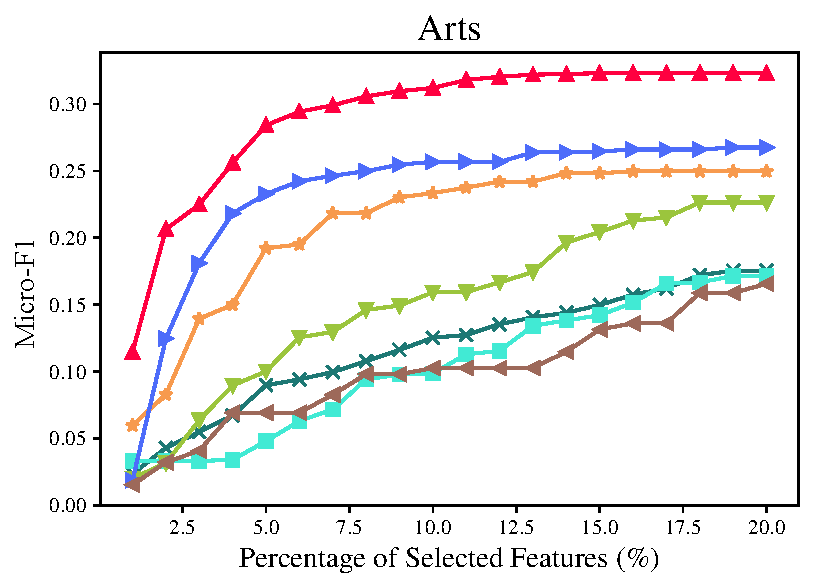
\includegraphics[width=0.43\textwidth]{figures/Micro/PSF(Arts).pdf}}
	{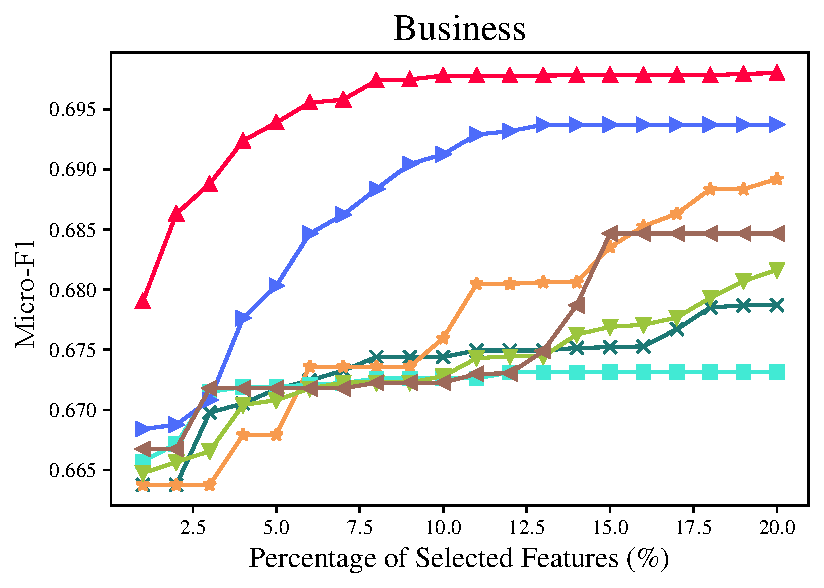
\includegraphics[width=0.43\textwidth]{figures/Micro/PSF(Business).pdf}}
	\\ 
	{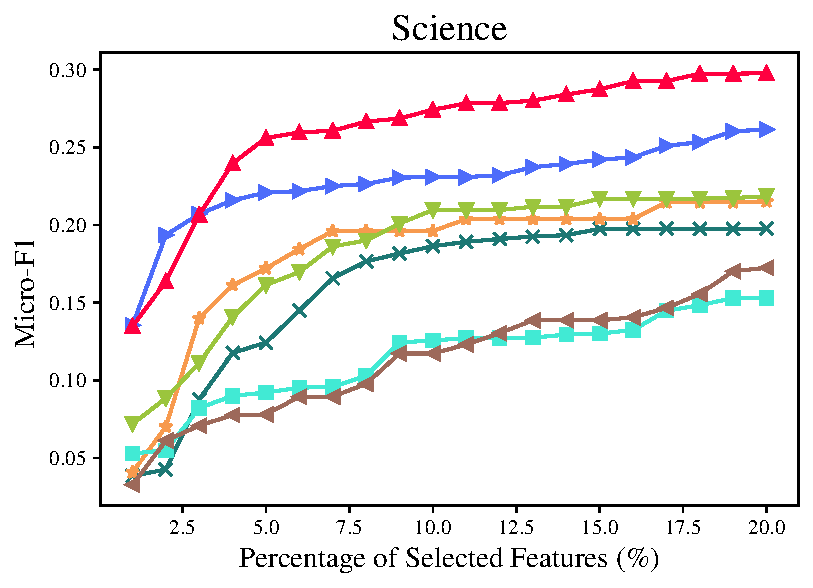
\includegraphics[width=0.43\textwidth]{figures/Micro/PSF(Science).pdf}}
	{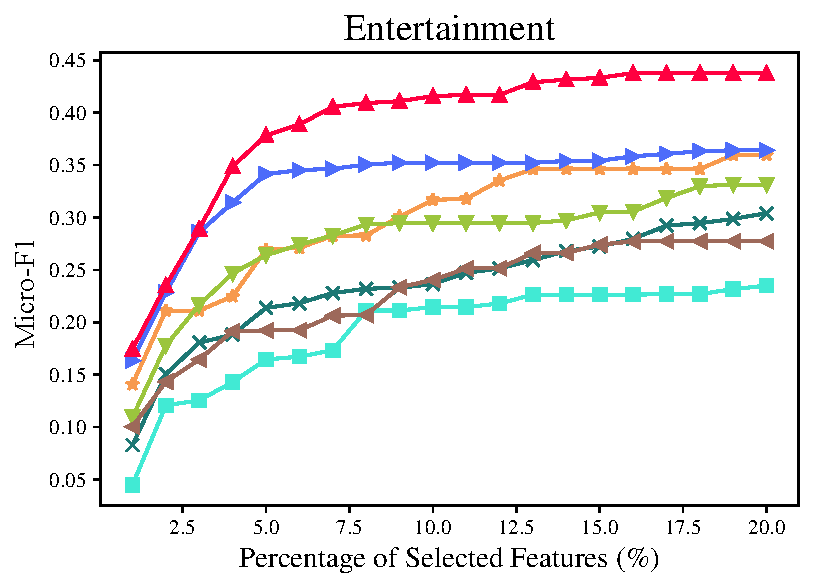
\includegraphics[width=0.43\textwidth]{figures/Micro/PSF(Entertainment).pdf}}
	{
\includegraphics[width=0.7\textwidth]{figures/Micro/FL.pdf}}
	\caption{نمودار درصد انتخاب ویژگی‌ها در معیار \lr{Micro-F1}}
	\label{fig:fmic}
\end{figure}
\begin{figure}
	\centering
	{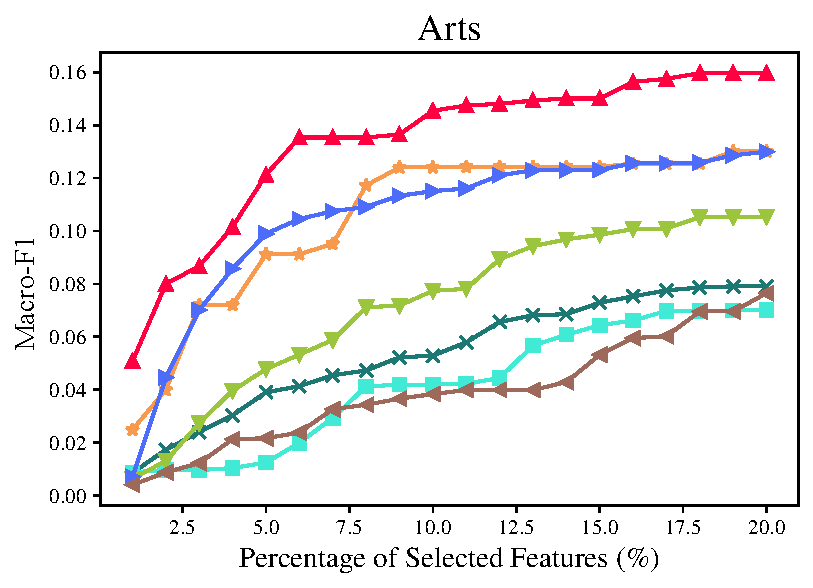
\includegraphics[width=0.43\textwidth]{figures/Macro/PSF(Arts).pdf}}
	{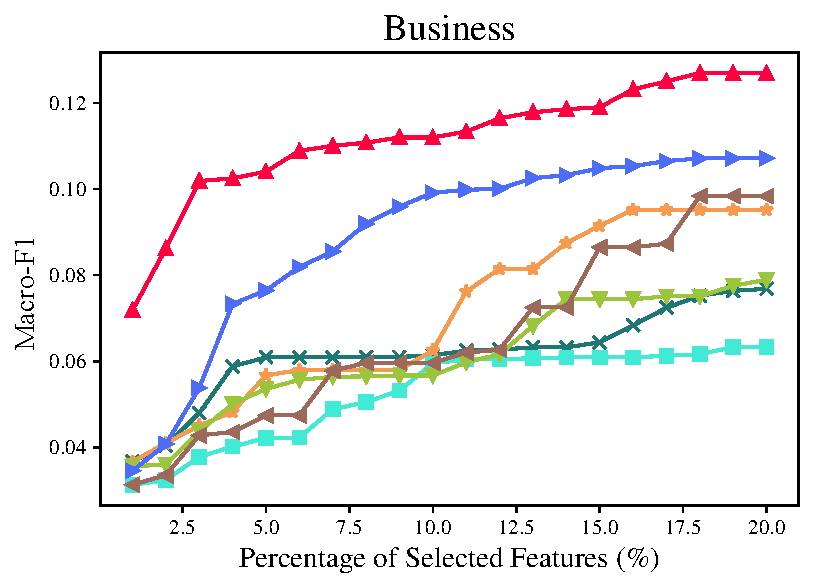
\includegraphics[width=0.43\textwidth]{figures/Macro/PSF(Business).pdf}}
	\\
	{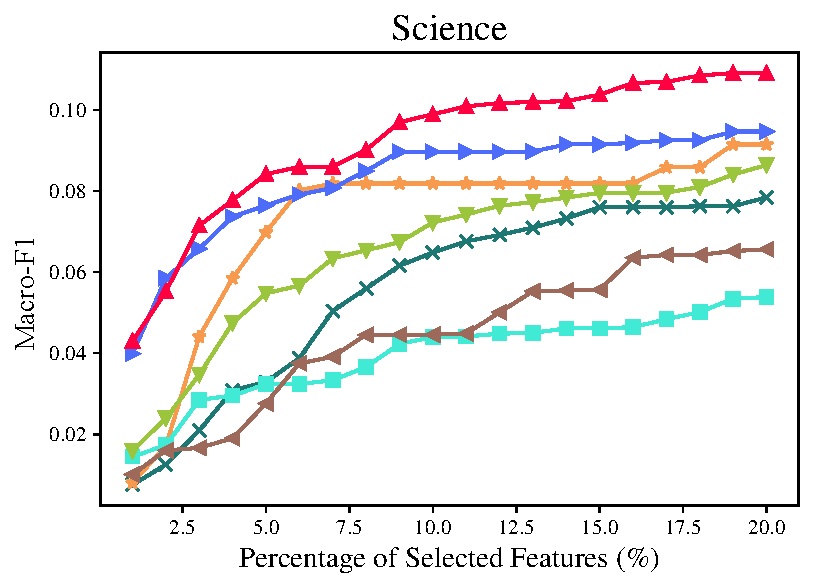
\includegraphics[width=0.43\textwidth]{figures/Macro/PSF(Science).pdf}}
	{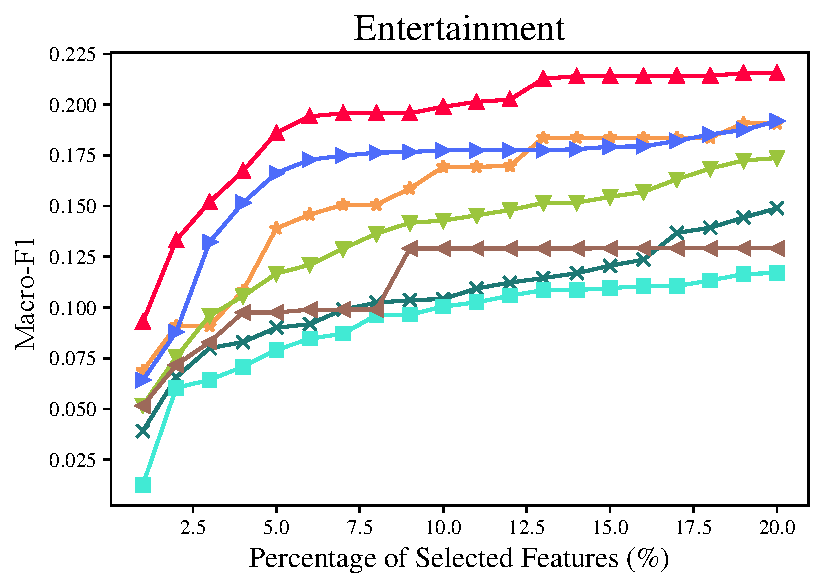
\includegraphics[width=0.43\textwidth]{figures/Macro/PSF(Entertainment).pdf}}
	{
\includegraphics[width=0.7\textwidth]{figures/Micro/FL.pdf}}
	\caption{نمودار درصد انتخاب ویژگی‌ها در معیار \lr{Macro-F1} }
	\label{fig:fmac}
\end{figure}
\begin{figure}
	\centering
	{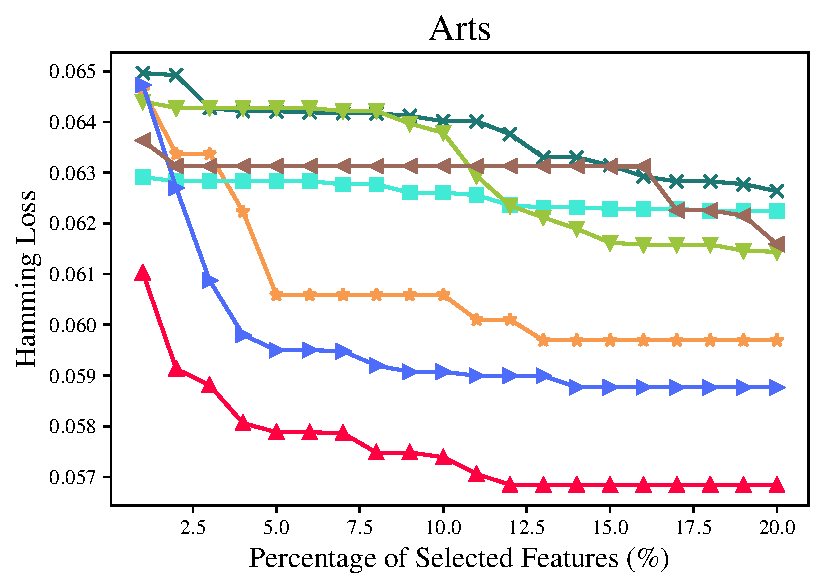
\includegraphics[width=0.43\textwidth]{figures/Hamming Loss/PSF(Arts).pdf}}
	{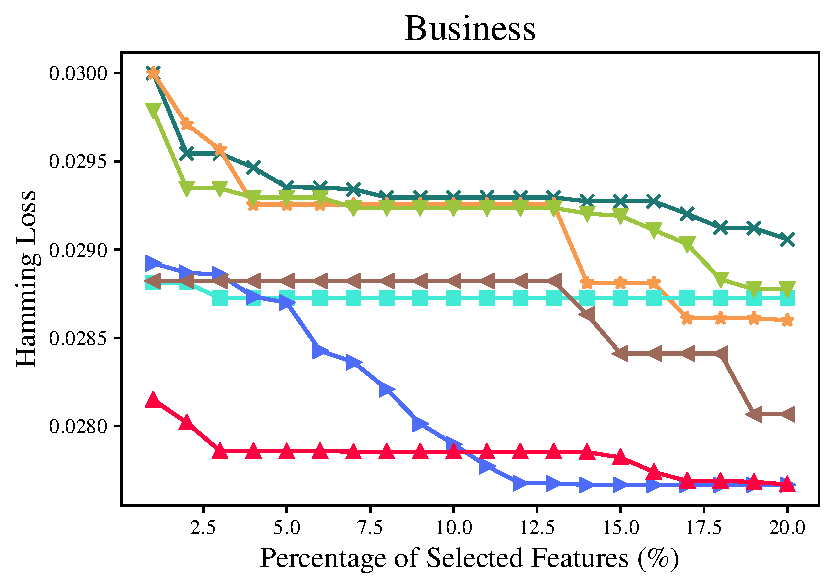
\includegraphics[width=0.43\textwidth]{figures/Hamming Loss/PSF(Business).pdf}}
	\\
	{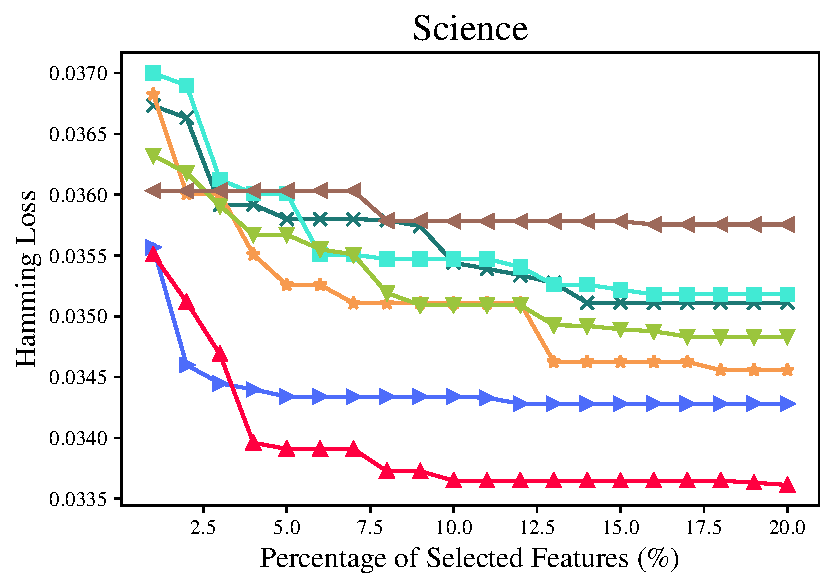
\includegraphics[width=0.43\textwidth]{figures/Hamming Loss/PSF(Science).pdf}}
	{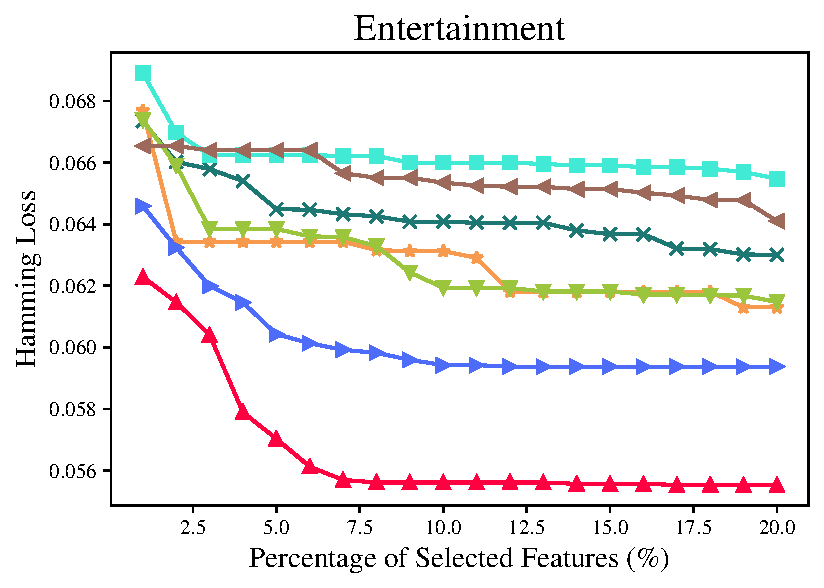
\includegraphics[width=0.43\textwidth]{figures/Hamming Loss/PSF(Entertainment).pdf}}
	{
\includegraphics[width=0.7\textwidth]{figures/Micro/FL.pdf}}
	\caption{نمودار درصد انتخاب ویژگی‌ها در معیار \lr{Hamming Loss} }
	\label{fig:fhml}
\end{figure}
\begin{figure}
	\centering
	{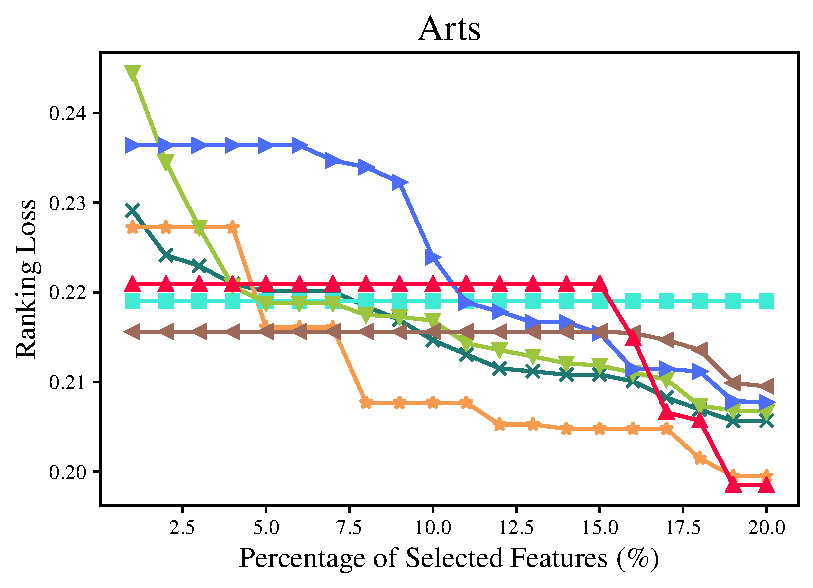
\includegraphics[width=0.43\textwidth]{figures/Ranking Loss/PSF(Arts).pdf}}
	{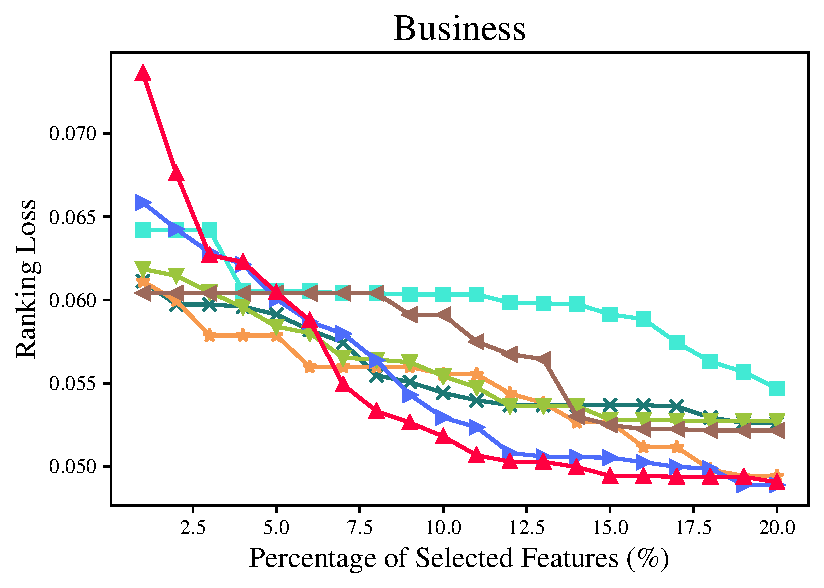
\includegraphics[width=0.43\textwidth]{figures/Ranking Loss/PSF(Business).pdf}}
	\\
	{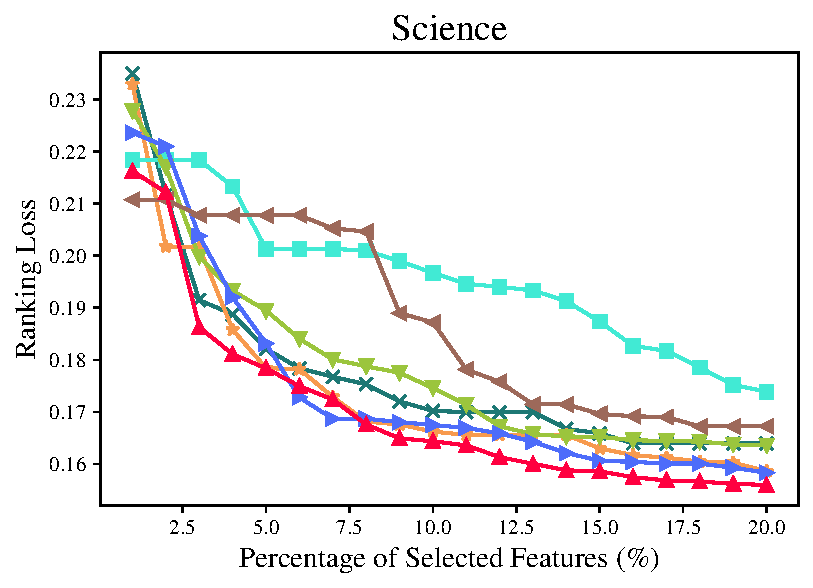
\includegraphics[width=0.43\textwidth]{figures/Ranking Loss/PSF(Science).pdf}}
	{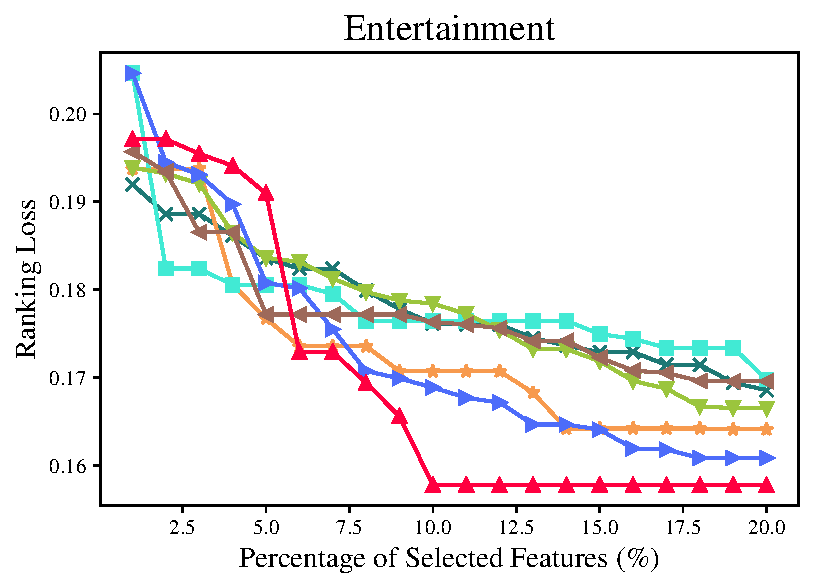
\includegraphics[width=0.43\textwidth]{figures/Ranking Loss/PSF(Entertainment).pdf}}
	{
\includegraphics[width=0.7\textwidth]{figures/Micro/FL.pdf}}
	\caption{\BNazTTN نمودار درصد انتخاب ویژگی‌ها در معیار \lr{Ranking Loss} }
	\label{fig:frnl}
\end{figure}
\section{تجزیه‌و‌تحلیل پارامترها}
در این بخش، تأثیر پارامترها، از جمله پارامتر منظم‌ساز گراف $\lambda_1$، پارامتر همبستگی برچسب سراسری و محلی $\lambda_2$، و پارامتر خلوتی $\lambda_3$ را تحلیل می‌کنیم. شکل‌های \ref{fig:P3D-MICMAC} و \ref{fig:PD3-HMLRNL} ‎\lr{Micro-F1}‎، ‎\lr{Macro-F1}‎، ‎\lr{Hamming Loss} و \lr{Ranking Loss } روش ما را با شش مجموعه‌داده $\lambda_1$، $\lambda_2،$ و $\lambda_3$ نشان می‌دهند. این شکل‌ها به‌صورت سه‌بعدی ترسیم شده‌اند، یعنی سه محور مربوط به $\lambda_1$، $\lambda_2$ و $\lambda_3$ است \cite{SALAHIAN2023119051}.

\begin{itemize}
	\item \subsubsection{ پارامتر $\lambda_1$}
	این پارامتر اثربخشی منظم‌ساز ‌خمینه فضای نمونه در مدل را کنترل  می‌کند. در این تحلیل پارامتر، مقادیر موجود در مجموعه
	\{100، 10، 1، 0/1، 0/01، 0\}
	برای پارامتر $\lambda_1$ در همه مجموعه‌های داده انتخاب شده‌اند. از شکل‌های \ref{fig:P3D-MICMAC}‎ و \ref{fig:PD3-HMLRNL} می‌توان نتیجه گرفت که مقدار بهینه برای این پارامتر معمولاً کمتر از ۱ است.
\end{itemize}
\begin{itemize}
	\item	\subsubsection{ پارامتر $\lambda_2$}
	این پارامتر اثربخشی همبستگی برچسب سراسری و محلی مدل را نشان می‌دهد و مقادیر تحلیل‌شده برای پارامتر $\lambda_2$
	\{0/1، 0/01، 0/001، \textsuperscript{6-}10، \textsuperscript{12-}10، 0\}
	هستند. همان‌طور که در شکل‌های \ref{fig:P3D-MICMAC} و \ref{fig:PD3-HMLRNL} مشاهده می‌کنیم، $\lambda_2$ با مقادیر کوچک معمولاً عملکرد بهتری را از نظر ‎\lr{Micro-F1}‎ و ‎\lr{Macro-F1}‎ نشان می‌دهد و با مقادیر بالا معمولاً از نظر معیارهای ‎\lr{Hamming Loss}‎ و ‎\lr{Coverage Error}‎ در چهار مجموعه‌داده عملکرد بهتری دارد. مقادیر نزدیک به صفر یا مقادیر بسیار بزرگ برای این پارامتر ممکن است عملکرد نسبتاً خوبی نداشته باشند.
\end{itemize}

\begin{itemize}
	\item	\subsubsection{ پارامتر $\lambda_3$}
	عبارت منظم‌ساز خلوت در ‎\lr{MLFS-GLOCAL}‎ توسط $\lambda_3$ کنترل می‌شود.  برای ‎پارامتر  $\lambda_3$‎
	محدوده مقادیر
	%\{0، 0.001، 0.1، 0.5، 1، 10\}
	\{10، 0/5، 0/1، 0/001، 0\}
	است. نتایج نشان می‌دهد که $\lambda_3$ یک کمیت ظریف است که معمولاً نیاز به تنظیم دقیق دارد. نتایج نشان می‌دهد که انتخاب مقادیر زیر 1 برای این پارامتر بهتر است.
\end{itemize}

\begin{figure}
	\centering
	\mysubfig{figures/Parameters3D/Health_Mic2.pdf}{Health}
	\mysubfig{figures/Parameters3D/Reference_Mic2.pdf}{Reference}
	\mysubfig{figures/Parameters3D/Society_Mic2.pdf}{Society}
	\\[0.5cm]
	\mysubfig{figures/Parameters3D/Health_Mac2.pdf}{Health}
	\mysubfig{figures/Parameters3D/Reference_Mac2.pdf}{Reference}
	\mysubfig{figures/Parameters3D/Society_Mac2.pdf}{Society}
	\\[0.3cm]
	\caption{تجزیه و تحلیل پارامترهای $\alpha$ و $\beta$ در مدل پیشنهادی }
	\label{fig:P3D-MICMAC}
\end{figure}
\begin{figure}
	\centering
	\mysubfig{figures/Parameters3D/Health_HML2.pdf}{Health}
	\mysubfig{figures/Parameters3D/Reference_HML2.pdf}{Reference}
	\mysubfig{figures/Parameters3D/Society_HML2.pdf}{Society}
	\\[0.5cm]
	\mysubfig{figures/Parameters3D/Health_RNL2.pdf}{Health}
	\mysubfig{figures/Parameters3D/Reference_RNL2.pdf}{Reference}
	\mysubfig{figures/Parameters3D/Society_RNL2.pdf}{Society}
	\\[0.3cm]
	\caption{تجزیه و تحلیل پارامترهای $\alpha$ و $\beta$ در مدل پیشنهادی }
	\label{fig:PD3-HMLRNL}
\end{figure}


%\begin{figure}
%	\centering
%	\captionsetup[subfigure]{position=top}
%	\subfloat[]{{\includegraphics[trim={0 1cm 0 0},clip,width=12cm]{figures/AUC Different Attack.eps}}}
%	\\
%	\subfloat[]{{\includegraphics[trim={9.25cm 2cm 0 0},clip,width=12.1cm]{figures/Precision Different Attack.eps}}}
%	\\
%	\includegraphics[height=0.7cm]{figures/Dataset name for different attack-pdf-crop.pdf}
%	\caption{نتایج ارزیابی در برابر حملات مختلف مهاجم}
%	\label{fig:4}
%\end{figure}


%\begin{figure}
%	\centering
%	\captionsetup[subfigure]{position=top}
%	\subfloat[C.elegans]{{\includegraphics[trim={0 0 0 1cm},clip,width=5cm]{figures/AUCCelegansneuralRemoveLink.eps}}}\quad
%	\subfloat[YeastL]{{\includegraphics[trim={0 0 0 1cm},clip,width=5cm]{figures/AUCYeastLRemoveLink.eps}}}
%	\\
%	\subfloat[ODLIS]{{\includegraphics[trim={0 0 0 1cm},clip,width=5cm]{figures/AUCODLISRemoveLink.eps}}}\quad
%	\subfloat[OpenFlights]{{\includegraphics[trim={0 0 0 1cm},clip,width=5cm]{figures/AUCOpenflightsRemoveLink.eps}}}
%	\\
%	\subfloat[SciMet]{{\includegraphics[trim={0 0 0 1cm},clip,width=5cm]{figures/AUCSciMetRemoveLink.eps}}}\quad
%	\subfloat[Power-US]{{\includegraphics[trim={0 0 0 1cm},clip,width=5cm]{figures/AUCPowerUSRemoveLink.eps}}}
%	\\
%	\includegraphics[height=0.47cm]{figures/Name-removed link-pdf-crop.pdf}
%	\caption{میزبه‌صورت مقاوم پذیری روش ‎\lr{LPANMF}‎ }
%	\label{fig:3}
%\end{figure}

\section{تحلیل همگرایی }
در این بخش، ما رفتار همگرایی\LTRfootnote{Convergence} مدل پیشنهادی \eqref{eq:BeOpt} را با انجام آزمایش‌هایی بر روی چهار مجموعه‌داده 
‎\lr{Arts}، \lr{Corel5k}، \lr{Health} و \lr{Reference}
ارزیابی می‌کنیم.
‎ الگوریتم \ref{alg:algorithm} را برای هر مجموعه‌داده با 600 تکرار اجرا می‌کنیم. مقدار تابع هدف را در برابر تعداد تکرارها در شکل \ref{fig:7} رسم کرده‌ایم تا نشان دهیم چگونه روش ما‌ همگرا می‌شود. همان‌طور که از شکل \ref{fig:7} مشاهده می‌شود، مقدار تابع هدف به سرعت و به‌طور پیوسته در تکرارهای اولیه کاهش می‌یابد، که نشان می‌دهد روش ما به سرعت به یک راه‌حل بهینه نزدیک می‌شود. در تکرارهای بعدی، مقدار تابع هدف بسیار کم تغییر می‌کند، و این نشان می‌دهد روش ما به یک راه‌حل تقریباً بهینه رسیده است. این بیانگر این می‌باشد که روش ارائه‌شده عملکرد همگرایی سریع و پایداری دارد.
\begin{figure}
	\centering
	\begin{minipage}[b]{0.48\textwidth}
		\centering
		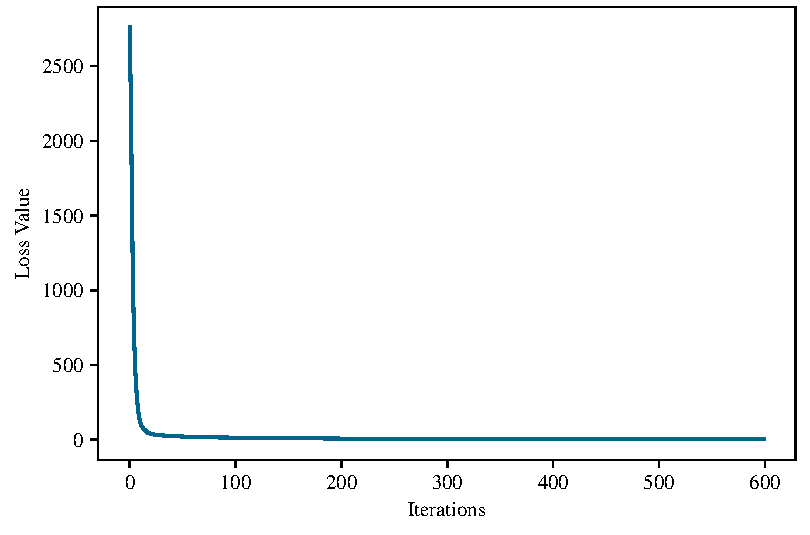
\includegraphics[width=\textwidth]{figures/Convergence/Convergence(Arts).pdf}
		\caption*{\centering Arts}
	\end{minipage}\hfill
	\begin{minipage}[b]{0.48\textwidth}
		\centering
		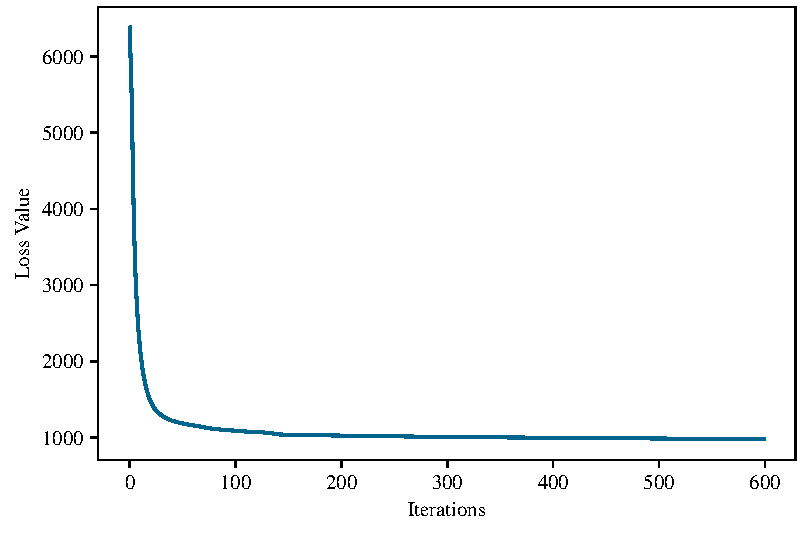
\includegraphics[width=\textwidth]{figures/Convergence/Convergence(Corel5k).pdf}
		\caption*{\centering Corel5k}
	\end{minipage}
	\\[0.5cm]
	\begin{minipage}[b]{0.48\textwidth}
		\centering
		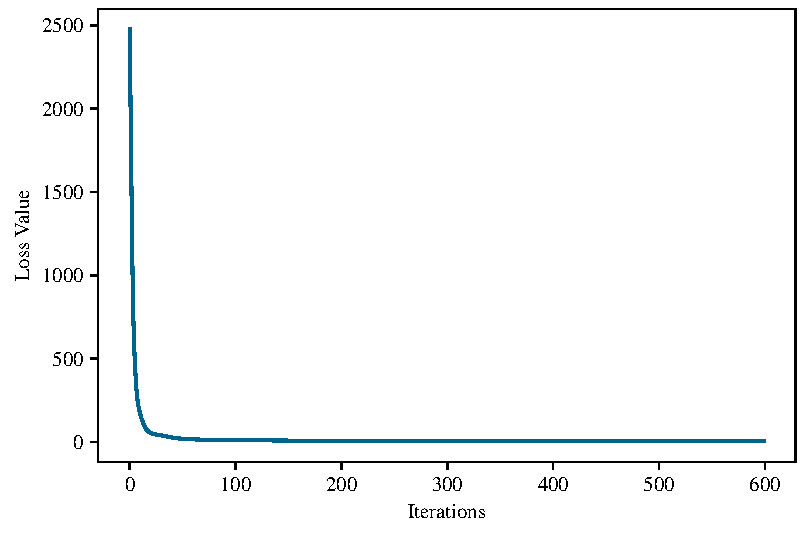
\includegraphics[width=\textwidth]{figures/Convergence/Convergence(Health).pdf}
		\caption*{\centering Health}
	\end{minipage}\hfill
	\begin{minipage}[b]{0.48\textwidth}
		\centering
		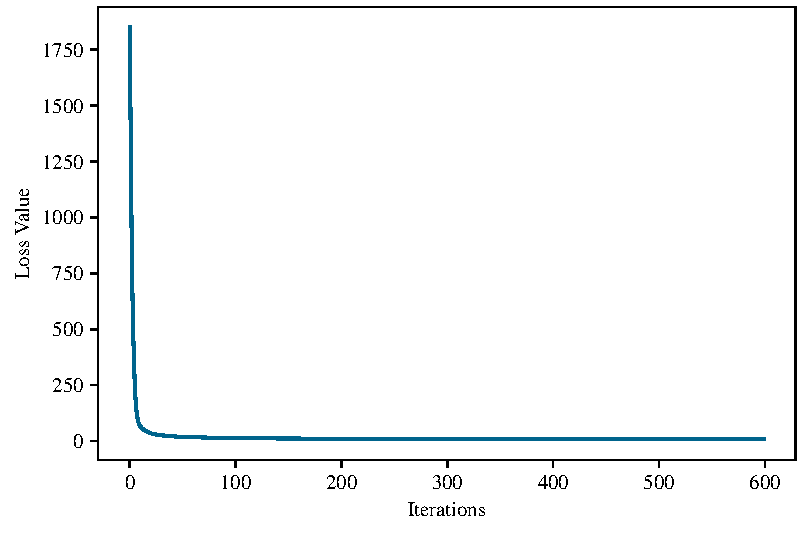
\includegraphics[width=\textwidth]{figures/Convergence/Convergence(Reference).pdf}
		\caption*{\centering Reference}
	\end{minipage}
	\caption{همگرایی مدل پیشنهادی \lr{(MLFS-GLOCAL)}}‎
	\label{fig:7}
\end{figure}

	
\titleformat{\chapter}[display]
{\normalfont\huge\bfseries\centering}
{\vspace*{6cm}{‎فصل پنجم}}{5pt}{\Huge}
\chapter{\rl{نتیجه گیری و کارهای آینده}}\label{sec5}
\thispagestyle{empty}
\newpage
\section{نتیجه‌گیری}
در این پایان‌نامه، ما یک روش جدید انتخاب ویژگی چندبرچسبه را با درنظر گرفتن همبستگی برچسب سراسری و محلی پیشنهاد کردیم. همبستگی برچسب سراسری به بهره‌برداری از ساختار زیربنایی فضای برچسب کمک می‌کند. این به مدل اجازه می‌دهد تا روابط و همبستگی‌های بین برچسب‌ها را یاد بگیرید، از سوی دیگر، همبستگی محلی برچسب به ارتباط بین برچسب‌ها در یک پارتیشن محلی خاص اشاره دارد. با درنظر گرفتن همبستگی بین برچسب‌ها و گنجاندن آن‌ها در بازنمایی ویژگی، مدل ویژگی‌هایی را شناسایی می‌کند که بیشترین ارتباط را با برچسب‌ها دارند. علاوه‌بر‌این، ‎\lr{MLFS-GLOCAL}‎ فضای مشترک بین ماتریس ویژگی و ماتریس برچسب را می‌آموزد تا همبستگی برچسب ضمنی را استخراج کند و انتخاب ویژگی را راهنمایی کند. این ماتریس کم‌بُعد از طریق منظم‌ساز چندگانه محدود می‌شود، به این معنی که ساختار محلی مشابهی با داده‌های اصلی دارد و  اطلاعات ارزشمند در داده‌ها حفظ می‌شود. یک الگوریتم تکراری مبتنی بر بهینه‌سازی متناوب برای حل تابع هدف با منظم‌ساز نُرم $\ell_{2,1} $ ایجاد شده است. در نهایت، آزمایش‌های گسترده بر روی مجموعه‌داده‌های چندبرچسبه انجام شده است تا اثربخشی ‎مدل‎ پیشنهادی را در برابر تعدادی از روش‌های انتخاب ویژگی پیشرفته نشان ‌دهد.
\section{پیشنهادهایی برای تحقیقات آتی}
روش‌های پیشنهادی آتی این پایانامه می‌تواند در زمینه‌‌های زیر باشد:
\begin{itemize} 
	
	\item 
	با توجه به اهمیت اطلاعات برچسب در دنیای واقعی می‌توان بر روی داده‌های نیمه‌نظارتی\LTRfootnote{Semi-supervised} \cite{CHAVOSHINEJAD2023109282,8324084} یا گم‌شده \cite{SEYEDI2023562} براساس همبستگی بین برچسب‌ها تمرکز کرد. 
	\item   می‌توان این روش پیشنهادی را بر روی داده‌های چندنمایه\LTRfootnote{Multi-view} چندبرچسبه توسعه داد که در آن داده‌ها با مجموعه ویژگی‌ها یا نماهای متعدد نشان داده می‌شوند و هر نمونه با چندین برچسب مرتبط می‌باشد.
\end{itemize}

%منابع و مأخذ
	\include{Chapters/6-Attachment}
	\settextfont{XB Niloofar}
% برای دانشجویانی که میخوان در پایان‌نامه خود از واژه نامه استفاده کنند دستورهای زیر را فعال نمایند.
%	\printglossary
%	\printabbreviation
%%%%%%%%%%%%%%%%%%%%%%%%%%%%%%%%%%%%
	\renewcommand{\bibname}{مراجع}	
{\normalfont\huge\bfseries\RTL}
\chapter*{\vspace*{8cm}مراجع}
\baselineskip=.6cm
\newpage
\begin{LTRitems}
	\resetlatinfont
	\begingroup
	\def\chapter*#1{}
	\bibliographystyle{IEEEtran}‎‎
	{\footnotesize\bibliography{Bibs/Ref}}
	\endgroup
\end{LTRitems}

\baselineskip=0.67cm
	
	% appendixes section...
	% برای دانشجویانی که از پایان‌نامه یا رساله خود مقاله استخراج کردن لطفا دستور زیر را فعال کنید و اطلاعات ان را در صفحه ی مربوطه وارد بفرمایند.
%	\include{Chapters/Dastavard}	
%%%%%%%%%%%%%%%%%%%%%%%%%%%%%%%%%%%%
	\begin{latin}
		% english abstract page...
		\newpage
		

%%%%%%%%%%%%%%%%%
%%%%%%%%%%%%%%%% چکیده به‌صورتگلیسی

%در چكيده به‌صورتگليسي، می‌باید عينا" متن چكيده فارسي به زببه‌صورت به‌صورتگليسي ترجمه شود.
\section*{Abstract}
In various application domains, high-dimensional multi-label data has become more prevalent, presenting two significant challenges: instances with high-dimensional features and a large number of labels. In the context of multi-label feature selection, the objective is to choose a subset of features from a given set that is highly pertinent for predicting multiple labels or categories associated with each instance. However, certain characteristics of multi-label classification, such as label dependencies and imbalanced label distribution, have often been overlooked although hold valuable insights for designing effective multi-label feature selection algorithms. In this research, we propose a feature selection model which exploits explicit global and local label correlations to select discriminative features across multiple labels. In addition, by representing the feature matrix and label matrix in a shared latent space, the model aims to capture the underlying correlations between features and labels. The shared representation can reveal common patterns or relationships that exist across multiple labels and features. An objective function involving $\ell_{2,1} $-norm regularization is formulated, and an alternating optimization-based iterative algorithm is designed to obtain the sparse coefficients for multi-label feature selection. The proposed method was evaluated on twelve real-world multi-label datasets using six evaluation metrics, through comprehensive experiments. The results indicate its effectiveness, surpassing that of several representative methods.	\\
%کلمات کلیدی به‌صورتگلیسی نیز عينا" ترجمه‌ی کلمات کلیدی فارسی هستند.\\
\noindent\textbf{Keywords:}
{feature selection, multi-label learning, label correlation, nonnegative matrix factorization}


%%%%%%%%%%%
%%%%%%%%%%%%%%
		\newpage
		% english cover page...
		
\thispagestyle{empty}
\begin{center}
	\vspace*{-1.5cm}
	\begin{figure}[ht]
		\centerline{
\includegraphics[height=2.5cm]{figures/UOK_LOGO.png}}
	\end{figure}
	\vspace*{-0.6cm}
	\textbf{{\Large University of Kurdistan}}
	\vspace*{-0.2cm}\\
	\textbf{{\large Faculty of Engineering}}
	\vspace*{-0.2cm}\\
	\textbf{Department of Computer Software Engineering}\\
	\vspace*{1cm}
	A Thesis Submitted to the Postgraduate Studies Office in Partial Fulfillment of the Requirements for the Degree of M.Sc. in Computer Engineering - Artificial Intelligence and Robotics\\
	\vspace*{0.5cm}
	\textbf{\Large{ Title:}}\\
	\textbf{
		{\Large
			Multi-Label Feature Selection by Exploiting Global and Local Label Correlation
		}
	}\\
	\vspace*{1cm}
	\textbf{By:}\\
	\textbf{
		{\Large
			Mohammad Faraji
		}
	}\\
\end{center}
The above thesis was evaluated and approved by the following members of the thesis committee --
%%%%%%%%%%%%%%%%%%
%mark …...…... and 		%برای دانشجویان دکتری باید نمره حتما وارد شود.
%%%%%%%%%%%%%%%%%%%%
\textbf{Excellent} quality on September 12, 2023}. 
\vspace*{-0.5cm}\\
%%%%
\begin{table}[!ht]
\centerline{
	%\scalebox{1}{
		\begin{tabular}{lllc}
			\underline{Position} & \underline{Name} & \underline{Acadmic Rank} & \underline{Signature} \\\\
			1. Supervisor:  & Dr. Fardin Akhlaghian Tab         & Associate Prof. &\\\\
			2. Advisor   :  &  Seyed Amjad Seyedi            &                 &\\\\
			2. External Examiner:  & Dr. Mohsen Ramezani Tab    & Assistant Prof. &\\\\
			3. Internal Examiner: &  Dr. Rojiar PirMohamadiani  & Assistant Prof. &\\\\
	\end{tabular}}
	%}
	\end{table}
	\\
	Head of Department:
	\hspace*{4.5cm}
	Faculty Graduate Coordinator:\\
		
%%%%%%%%%% صفحه عنوبه‌صورت انگلیسی و پشت جلد
\newpage
\thispagestyle{empty}
\begin{center}
		\vspace*{-1.5cm}
	\begin{figure}[ht]
		\centerline{
\includegraphics[height=2.5cm]{figures/UOK_LOGO.png}}
	\end{figure}
	\vspace*{-0.6cm}
	\textbf{{\Large University of Kurdistan}}
	\vspace*{-0.2cm}\\
	\textbf{{\large Faculty of Engineering}}
	\vspace*{-0.2cm}\\
	\textbf{Department of Computer Software Engineering}\\
	\vspace*{1cm}
A Thesis Submitted in Partial Fulfillment of the Requirements for the Degree\\
 of M.Sc. in  Computer Engineering – Artificial Intelligence and Robotics\\
	\vspace*{0.5cm}
	\textbf{\Large{Title:}}\\
	\textbf{{\Large
			Multi-Label Feature Selection by Exploiting Global and Local Label Correlation
	}}\\
	\vspace*{1cm}
	\textbf{By:}\\
	\textbf{
		{\Large
			Mohammad Faraji
		}
	}\\
	\vspace*{1cm}			
	\textbf{Supervisor:}\\
	\textbf{
		{\Large
			Dr. Fardin Akhlaghian Tab
		}
	}\\
	\vspace*{1cm}			
	\textbf{Advisor:}\\
	\textbf{
		{\Large
			Seyed Amjad Seyedi
		}
	}\\
	\vspace*{2cm}			
	\textbf{{Septamber 2023}}
\end{center}





%%%%%%%%%%%%%%%%%%%%%%%%%%%%%%%%%%%%%%%%%%%%%%%%%%%%%%%%%%%%%%%%%%%%%%%%%%%%%%%%%%%%%%%%%%%%%%%%%%%%%%%%%%%%%%%%%%%%%%%%%%%%%%%%%%%%%%%%%%%%%%%%%%%%%%%%%%%%%%%%%%%%%%%%%%%%%%%%%%%%
%%%%%%%%%%%%%%%%%%%%%%%%%%%%%%%%%%%%%%%%%%%%%%%%%%%%%%%%%%%%%%%%%%%%%%%%%%%%%%%%% Guide Section %%%%%%%%%%%%%%%%%%%%%%%%%%%%%%%%%%%%%%%%%%%%%%%%%%%%%%%%%%%%%%%%%%%%%%%%%%%%%%%%%%%%

%Academic Ranks:
%	Professor/ Associate Professor/ Assistant Professor 


%Leve of Scores:

% 1. 19~20 -----------> Excellent
% 2. 18~19 -----------> Very Good
% 3. 17~18 -----------> Good

	\end{latin}	
	\newpage
	\BNazF
\section*{\textcolor{red}{\textbf{تصویر انگلیسی جلد در این صفحه قرار میگیرد.}}}
\thispagestyle{empty}
\DraftwatermarkOptions{stamp=false}
	

\end{document}
%%%%%%%%%%%%%%%%%%%%%%%%%%%%%% 